%%%%%%%%%%%%%%%%%%%%%%%%%%%%%%%%%%%%%%%%%%%%%%%%%%%%%%%%%%%%%%%%%%%%%
%%                                                                 %%
%% Please do not use \input{...} to include other tex files.       %%
%% Submit your LaTeX manuscript as one .tex document.              %%
%%                                                                 %%
%% All additional figures and files should be attached             %%
%% separately and not embedded in the \TeX\ document itself.       %%
%%                                                                 %%
%%%%%%%%%%%%%%%%%%%%%%%%%%%%%%%%%%%%%%%%%%%%%%%%%%%%%%%%%%%%%%%%%%%%%

%%\documentclass[referee,sn-basic]{sn-jnl}% referee option is meant for double line spacing

%%=======================================================%%
%% to print line numbers in the margin use lineno option %%
%%=======================================================%%

%%\documentclass[lineno,sn-basic]{sn-jnl}% Basic Springer Nature Reference Style/Chemistry Reference Style

%%======================================================%%
%% to compile with pdflatex/xelatex use pdflatex option %%
%%======================================================%%

%%\documentclass[pdflatex,sn-basic]{sn-jnl}% Basic Springer Nature Reference Style/Chemistry Reference Style

%%\documentclass[sn-basic]{sn-jnl}% Basic Springer Nature Reference Style/Chemistry Reference Style
\documentclass[sn-mathphys]{sn-jnl}% Math and Physical Sciences Reference Style
%%\documentclass[sn-aps]{sn-jnl}% American Physical Society (APS) Reference Style
%%\documentclass[sn-vancouver]{sn-jnl}% Vancouver Reference Style
%%\documentclass[sn-apa]{sn-jnl}% APA Reference Style
%%\documentclass[sn-chicago]{sn-jnl}% Chicago-based Humanities Reference Style
%%\documentclass[sn-standardnature]{sn-jnl}% Standard Nature Portfolio Reference Style
%\documentclass[default]{sn-jnl}% Default
%%\documentclass[default,iicol]{sn-jnl}% Default with double column layout

%%%% Standard Packages
%%<additional latex packages if required can be included here>
%%%%

%%%%%=============================================================================%%%%
%%%%  Remarks: This template is provided to aid authors with the preparation
%%%%  of original research articles intended for submission to journals published 
%%%%  by Springer Nature. The guidance has been prepared in partnership with 
%%%%  production teams to conform to Springer Nature technical requirements. 
%%%%  Editorial and presentation requirements differ among journal portfolios and 
%%%%  research disciplines. You may find sections in this template are irrelevant 
%%%%  to your work and are empowered to omit any such section if allowed by the 
%%%%  journal you intend to submit to. The submission guidelines and policies 
%%%%  of the journal take precedence. A detailed User Manual is available in the 
%%%%  template package for technical guidance.
%%%%%=============================================================================%%%%
%\usepackage{cite}
\usepackage{amsmath,amssymb,amsfonts}
%\usepackage{algorithmic}
\usepackage{graphicx}
%\usepackage{textcomp}
\usepackage{color}

\def\bbeta{{\boldsymbol{\beta}}}

\jyear{2021}%

%% as per the requirement new theorem styles can be included as shown below
\theoremstyle{thmstyleone}%
\newtheorem{theorem}{Theorem}%  meant for continuous numbers
%%\newtheorem{theorem}{Theorem}[section]% meant for sectionwise numbers
%% optional argument [theorem] produces theorem numbering sequence instead of independent numbers for Proposition
\newtheorem{proposition}[theorem]{Proposition}% 
%%\newtheorem{proposition}{Proposition}% to get separate numbers for theorem and proposition etc.

\theoremstyle{thmstyletwo}%
\newtheorem{example}{Example}%
\newtheorem{remark}{Remark}%

\theoremstyle{thmstylethree}%
\newtheorem{definition}{Definition}%

\raggedbottom
%%\unnumbered% uncomment this for unnumbered level heads

\begin{document}

\title[Article Title]{Statistical supervised learning with engineering data: A case study of low frequency noise measured on semiconductor devices}

%%=============================================================%%
%% Prefix	-> \pfx{Dr}
%% GivenName	-> \fnm{Joergen W.}
%% Particle	-> \spfx{van der} -> surname prefix
%% FamilyName	-> \sur{Ploeg}
%% Suffix	-> \sfx{IV}
%% NatureName	-> \tanm{Poet Laureate} -> Title after name
%% Degrees	-> \dgr{MSc, PhD}
%% \author*[1,2]{\pfx{Dr} \fnm{Joergen W.} \spfx{van der} \sur{Ploeg} \sfx{IV} \tanm{Poet Laureate} 
%%                 \dgr{MSc, PhD}}\email{iauthor@gmail.com}
%%=============================================================%%

\author*[1]{\fnm{Mar\'ia Luz} \sur{G\'amiz}}\email{mgamiz@ugr.es}
\equalcont{These authors contributed equally to this work.}

\author[1]{\fnm{Anton} \sur{Kal\'en}}\email{anton.kalen@uvigo.es}
\equalcont{These authors contributed equally to this work.}

\author[2]{\fnm{Rafael} \sur{Nozal-Ca\~nadas}}\email{rca015@uit.no}
\equalcont{These authors contributed equally to this work.}

\author[1]{\fnm{Roc\'io} \sur{Raya-Miranda}}\email{rraya@ugr.es}
\equalcont{These authors contributed equally to this work.}

\affil*[1]{\orgdiv{Department of Statistics and O.R.}, \orgname{University of Granada},\country{Spain}}%, \orgaddress{\street{Street}, \city{City}, \postcode{100190}, \state{State}, \country{Country}}}

\affil[2]{\orgdiv{Department of Computer Science}, \orgname{UiT-The Artic University of Norway},\country{Norway}}%, \orgaddress{\street{Street}, \city{City}, \postcode{10587}, \state{State}, \country{Country}}}

%\affil[3]{\orgdiv{Department}, \orgname{Organization}, \orgaddress{\street{Street}, \city{City}, \postcode{610101}, \state{State}, \country{Country}}}

%%==================================%%
%% sample for unstructured abstract %%
%%==================================%%

\abstract{Our practical motivation is the analysis of potential correlations between spectral noise current and threshold voltage from common on-wafer MOSFETs. The usual strategy leads to the use of standard techniques based on Normal linear regression easily accessible in all statistical software (both free or commercial). 
However, these statistical methods are not appropriate because the assumptions they lie on are not met. More sophisticated methods are required. A new strategy based on the most novel nonparametric techniques which are data-driven and thus free from questionable parametric assumptions is proposed. A backfitting algorithm accounting for random effects and nonparametric regression is designed and implemented. The nature of the correlation between threshold voltage and noise is examined by conducting a statistical test, which is based on a novel technique that summarizes in a color map all the relevant information of the data. The way the results are presented in the plot makes it easy for a non-expert in data analysis to understand what is underlying. The good performance of the method is proven through simulations and it is applied to a data case in a field where these modern statistical techniques are novel and result very efficient. }
%We apply the method to the available data and carry out an extensive simulation study to prove the good performance of the algorithm.}



\keywords{1/f Noise, Backfitting Algorithm, Bootstrap, MOSFET, SiZer Map, Statistical Modeling.}

%%\pacs[JEL Classification]{D8, H51}

%%\pacs[MSC Classification]{35A01, 65L10, 65L12, 65L20, 65L70}

\maketitle

\section{Introduction}\label{sec1}

In the last 50 years, the Semiconductor Industry has decreased the dimensions of transistors significantly to almost atomic dimensions with the aim of increasing the production of transistors with time. This down-scaling strategy is leading to serious consequences. On the one hand, transistors become cheaper to manufacture, are able to work at faster switching rates, and consume less power. On the other hand, due to, among other causes, production defects, variability is being induced thus producing signal fluctuations, see \cite{Schroder2006} and \cite{Tsividis1998}. These phenomena are not avoidable at all and are becoming more and more important for the Semiconductor Industry. One of the most important consequences is that the  scaling of MOS transistors has decreased the current signals down to the level where they are not significantly higher than the fluctuations induced by carrier trapping phenomena, \cite{RMGRO2016}.  Therefore, a lot of effort has been made to improve the quality and to decrease noise inside the devices. Noise is a stochastic signal and unpredictable, therefore it is necessary to use statistical methods to analyze its behavior. Any tentative to understand the random behavior of the underlying phenomenon can allow to undertake further improvements, see \cite{Tetal2015}, \cite{Betal2016} and \cite{Betal2020}, among others. One interesting investigation line is to analyze the problem from a statistical perspective and in this sense the study of potential correlations between the switching threshold voltage and noise characteristics is of great importance, as considered in \cite{Duty2016}, and yet it has received little attention in the current literature.

The main concern of this paper is to explore possible correlations between spectral noise current and threshold voltage measured on common on-wafer MOSFETs (Metal Oxide Semiconductor Field Effect Transistor) and to explain its nature. The response variable is noise power level, which is dominated by the flicker noise that appears in a certain 1/f slope in the frequency domain. The goal is to build a model able of quantifying the effect of the threshold voltage on this noise signal. 

Although the literature on stochastic models for explaining the random behavior of low frequency noise is not short (see \cite{Petal2019}, \cite{WK2020}, \cite{Betal2016}, \cite{Betal2020}), however there are not many studies specifically focused on the relationship noise-voltage from a statistical learning point of view, that is, based on data. This is where the statistician can get into the game with the aim of adapting powerful machine learning techniques that have  been far demonstrated their efficacy both theoretic and practically and bringing them to this particular application field of Physics. The study for this paper has been developed  based on a sample obtained as follows. For each transistor on the wafer, a unique measurement of threshold voltage is determined. However the noise is measured at different frequency values for each transistor. As a result, we obtain for each transistor various noise measurements, one for each fixed frequency level. 

As explained in \cite{Schroder2006} to characterize a MOSFET it is very useful to observe the point at which the channel is filled with enough carriers to let an ``appreciable'' drain current flow. The characteristic switching point or gate voltage is called the {\it threshold voltage} ($V_{th}$). For the extraction of the threshold voltage of a transistor several methods can be used in practice. The data analyzed in this paper have been obtained by the second derivative method or trans-conductance method.
% Shortly, in this method, the drain current is represented as a function of the gate voltage. A transistor working properly presents an increasing exponential curve. The threshold voltage is the value of the gate voltage where the second derivative of the curve is zero.
Each transistor, on a silicon wafer, has a specific threshold voltage which usually has a small variability. 
In the processing of MOS Device Characterization, it is one of the most important and commonly used factors to characterize semiconductor devices, \cite{Duty2016}, \cite{Schroder2006}. The levels can vary from transistor to transistor. Even on the same wafer, there exist various threshold voltages for the transistors. %The threshold voltage depends strongly on several factors that affect the wafer production process, such as the level of doping or the amount of impurities \cite{Tsividis1998}.

Noise is normally understood as a spontaneous fluctuation in current or in voltage. Different types of noise have been observed in any electronic solid state device, including semiconductors devices like MOSFETs. The flicker noise or 1/f noise appears mostly in the low frequency range, where it dominates the power density spectrum. This kind of noise is associated with the imperfection in the process of fabrication and with material defects. It is observed under bias conditions in all semiconductor devices and usually the power density spectrum has a characteristic $1decade/1decade$ slope in the frequency domain. The physical origins of flicker noise are not definitively proven. However there exists strong evidence that 1/f noise is caused by the number of fluctuations of the carriers and not, as claimed in the past, by the mobility fluctuations of the carriers. The 1/f noise is then related to the random trapping and detrapping events of charged traps near to the silicon oxide surface $SiO_2$ (see \cite{HKHC1990}).\ 

Noise measurement of MOSFETs can be performed at fixed bias points, that is, applying fixed voltage or current signals at the gate and drain of the transistor. The measurements are registered during  a certain period of time, transformed using the Fast Fourier Transformation into the frequency domain, and afterward converted into the power density spectrum (PSD), \cite{Duty2016}. These measurements require high accuracy and high resolution to determine the differences between the observations. Depending on the device, the resolution unit can be in the nano ampere range. The experiment providing the data analyzed here  has been performed in the Laboratory of Nanoelectronics in the Research Centre for Information and Communications Technologies (CITIC-UGR) at the University of Granada (Spain). Specific equipment with high requirements concerning the accuracy, resolution and general connection has been used. Afterward, the data have been processed developing original scripts in the programming environment R to implement the statistical methods proposed in this paper to process the data. \

%As mentioned above, the general motivation of this paper is to ascertain possible correlations between the characteristic threshold voltage and the noise power level of the transistors on a wafer based on a sample of noise measurements at various levels of frequency. We believe that these insights can eventually help to improve the production process and further the reliability of MOSFET transistors.  


%%%%%%%%%%%%%%%%%

This paper is organized as follows. Section \ref{sec:dataset} describes the dataset and a first approach based on classical statistics. In Section \ref{sec:model} our proposal to analyze the data is presented.  Section \ref{sec:result} gives numerical results. A useful graphic test is shown in Section \ref{sec:sizer} and finally the conclusions are in Section \ref{sec:concl}.

%%%%%%%%%%%%%%%%%%%%%%%%
\section{First approach based on the classical linear model} \label{sec:dataset}

In the context of integrated circuits, a $DIE$ is a rectangular pattern (a small block of semiconducting material) on a wafer that contains circuitry to perform a specific function.  
The dataset analyzed in this paper has been provided by an experimental study of {\ttfamily{ Wafer PH1WY107MXA4 Alias} } {$1D-11$} on Nanoelectronics Laboratory probe-station $\# 2$ ({\ttfamily{SUSS PA300PSMA}}). \\
The sample units are $DIE$s which are physically  located on a wafer that is cut (diced) into many pieces (cells) each containing one copy of the circuit. So the wafer is seen as a square grid where each unit occupies a cell localized in terms of its spatial coordinates. 
Figure $\ref{fig:wafer}$ (left panel) presents the spatial arrangement of the units sampled in the grid (wafer). On the right panel a pictogram of the values of $V_{th}$ measured for each $DIE$. Empty cells represent missing data.
It is suspected that measures associated to  adjacent cells are correlated and that the correlations decreases as the distance between cells increases. Therefore spatial autocorrelation could be taken into account and therefore certain geo-statistical techniques are welcome. This aspect is out of the scope of this work and will be considered in a future research.%\footnote{Esta correlacion no la tenemos en cuenta en principio en el paper, lo dejo de momento para no perderlo de vista totalmente}
\begin{figure}[ht]
	\centering
		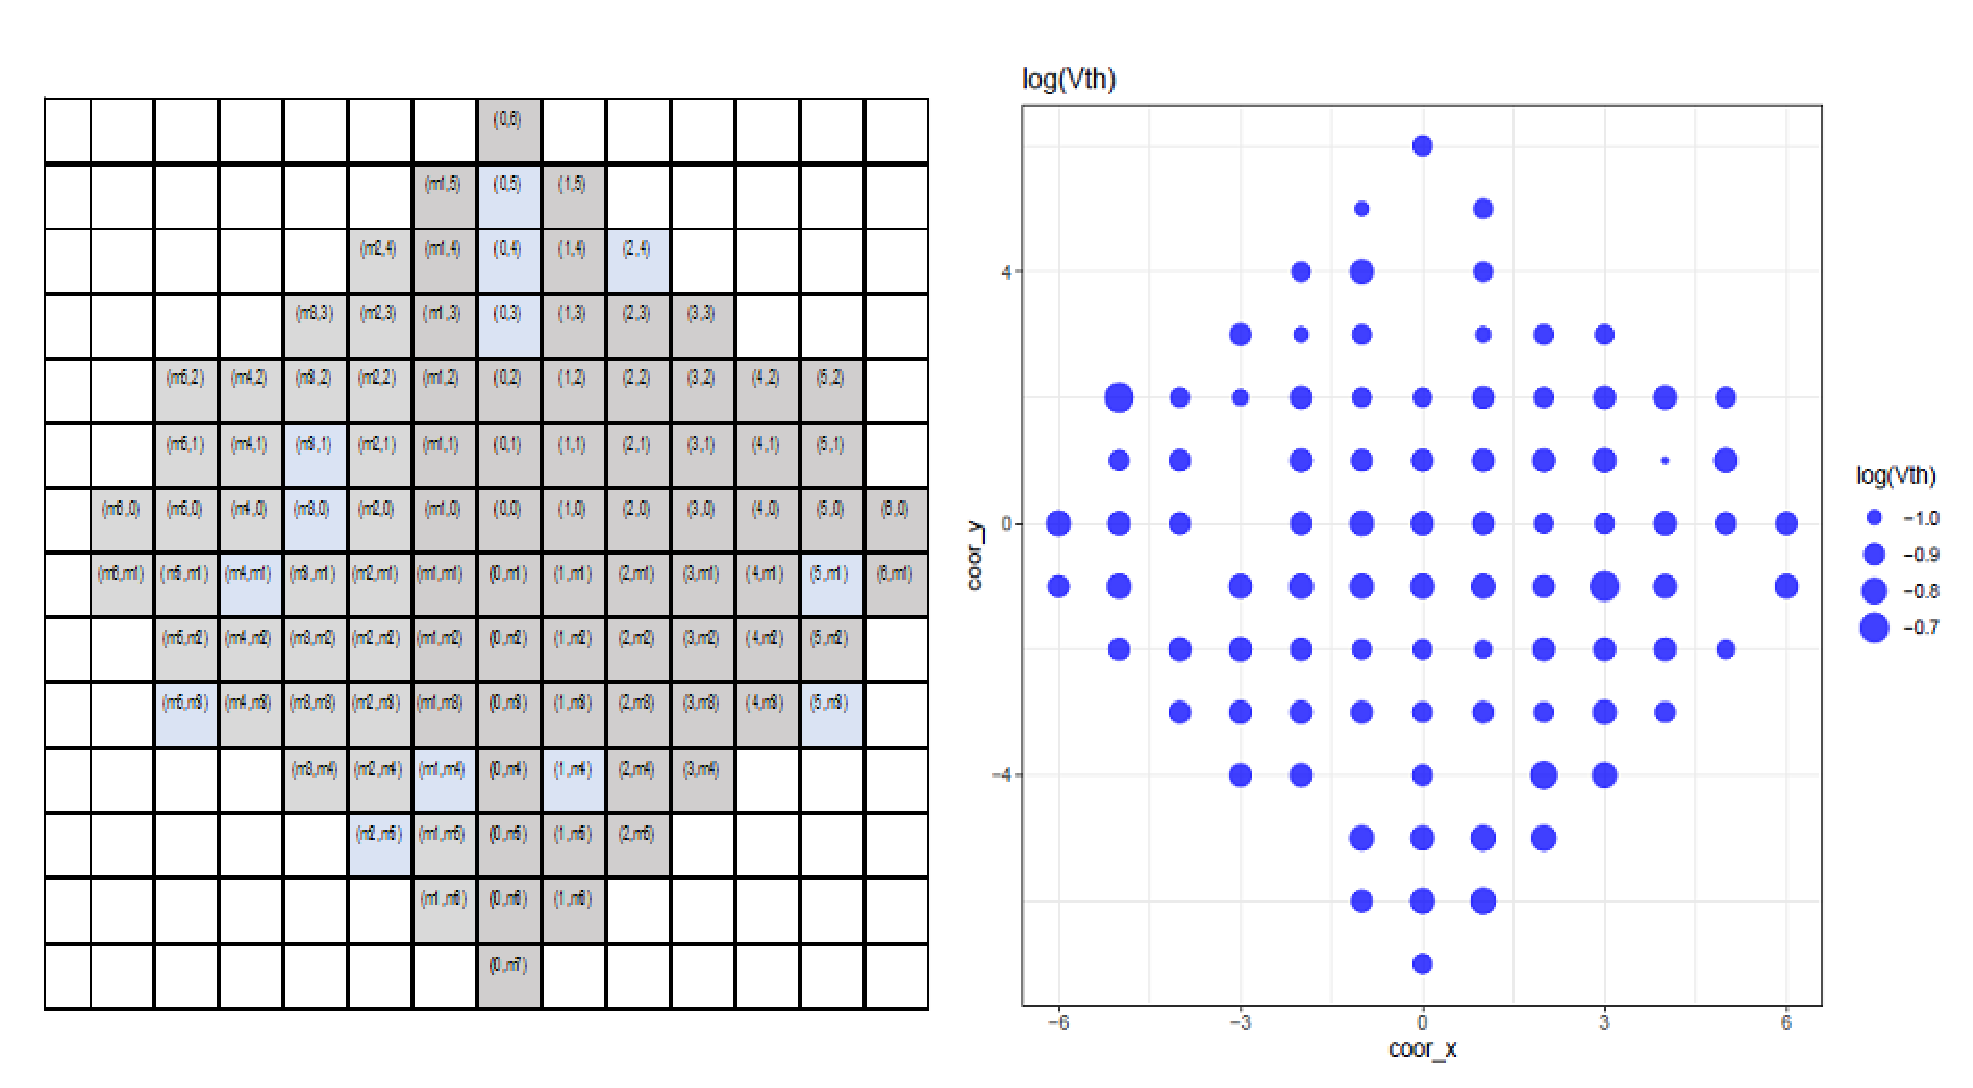
\includegraphics[width=0.7\textwidth]{Fig1_wafer2.eps}
	\caption{{\it Left panel}: Spatial location of $DIE$s within the wafer. Blue cells are missing data. {\it Right panel}:Pictogram of the threshold voltage $V_{th}$ at each location in the wafer.}
	\label{fig:wafer}
\end{figure}



In this section, a first approach to the data based on classic models which rely on strong assumptions, such as normality and independence of the measurements is carried out. We will see that these assumptions are not met by the data and can lead us to wrong conclusions. In any case, we will have into account the results as a start point for further and more sophisticated analysis developed in later sections of this paper.
%%%%%%%%%%%%%%%%%%%%%%%%%%%%%%%%%%%%%%%%%%%%%%%%%%%%%%%%%%%%%%%%%%%%%%%%%%%%%%%%%%%%%%%%%%%%%%%%%%%%%%%%%%%%%%%%%%%%%%%%%%%%%%%%%%%%%%%%%%%%
\subsection{Some descriptive plots}
A sample of $N = 1068$ observations is available. On the one hand, there are $Noise$ measurements taken on-wafer at a total of $n=89$ locations, each one containing one  $DIE$. In the sequel sampled units are referred as $DIE$s. The $Noise$ information is provided in the frequency domain at three different levels. Specifically, it is considered $Freq$= 100Hz, 1000Hz, 10000Hz. The bias conditions are fixed at four levels determined by all combinations of two values of drain and gate voltage, which are: $V_d$=0.5v, 1v, and $V_g$=0.5v, 1v. Therefore, we have in total 12 observations related to $Noise$ for each item or $DIE$. Besides, the value of  the threshold voltage $V_{th}$ is registered for each $DIE$. Unlike the variable $Noise$, the variable $V_{th}$ is an intrinsic feature of the item and, as such, there is one unique record per $DIE$.\\

With respect to the $Noise$ variable, we have, from the statistical point of view, a three-factorial design with correlated data (this aspect will be discussed later), as each subject is tested for all combinations of the levels of the three factors: $Freq$, $V_d$ and {\it Vg}. In other words, we have a factorial repeated measures design, \cite{BHN2000}.\\

Firstly we notice that the measures of  $Noise$ are strongly skewed to the right, so we recommend to consider this variable in the logarithmic scale.

Figure \ref{fig:trellis2} presents a bivariate trellis diagram for $\log Noise$ versus $Freq$ and for all combinations of levels of $V_d$ and {\it Vg}.

The variation in $V_d$ does not seem to affect the behavior of $Noise$ along the observations, or it has a small influence, which leads to think that this factor does not have a significant effect on the response $Noise$.  

We notice a remarkable decreasing trend of $Noise$ as $Freq$ increases. In the same way, smaller values of $Noise$ are related to the highest level of $V_g$. That is, we detect an inverse relationship between these two factors and the response, in other words, a decreasing relationship between $Freq-Noise$ as well as $V_g-Noise$ seems to be detected. 
%%%%%%%%%%%%%%%%%%%%%%%%%%%%%%%
\begin{figure}[ht]
	\centerline{
		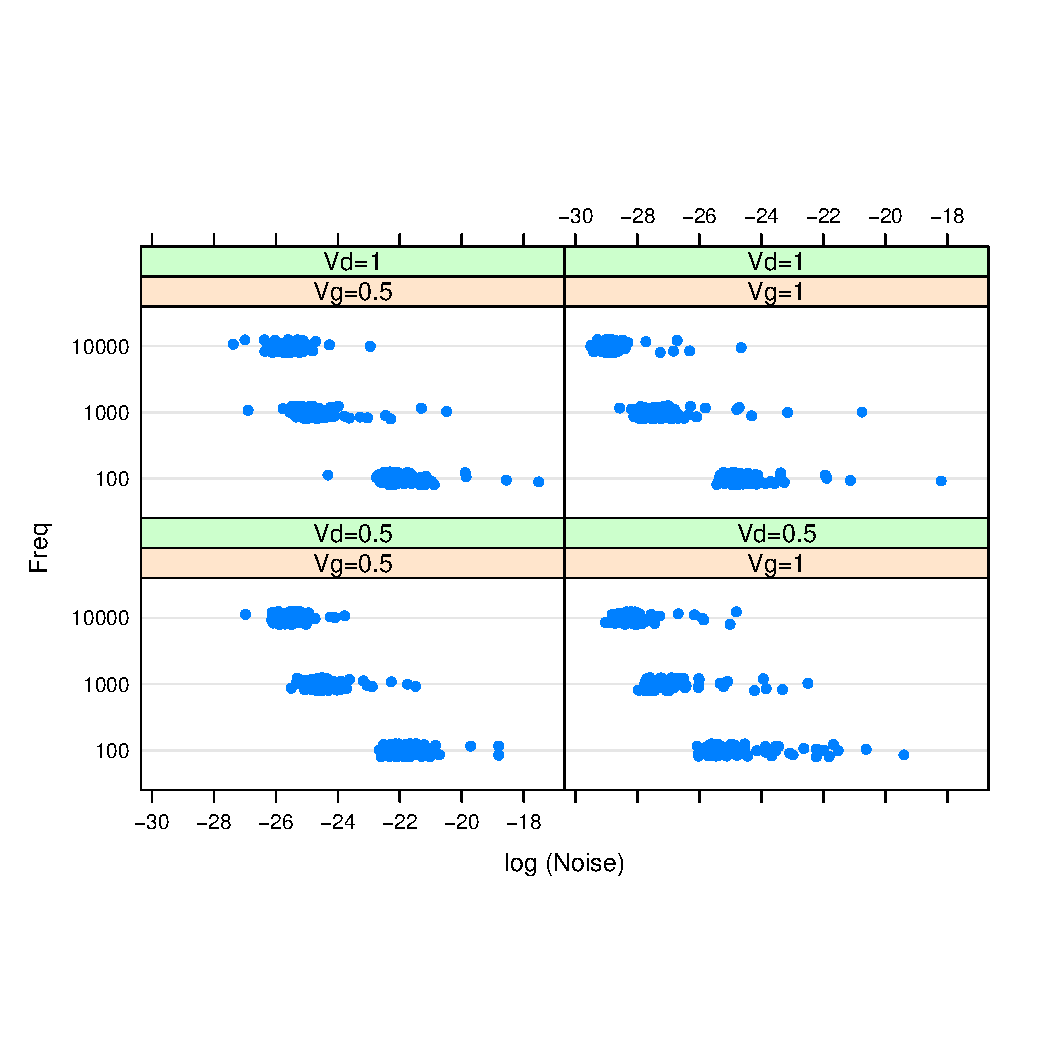
\includegraphics[width=0.6\textwidth]{Fig2_trellis2.eps}}
	\caption{Exploratory analysis: Trellis diagram. }
	\label{fig:trellis2}
\end{figure}


%To have one more visualization of the data we present a $spaghetti$ plot in Figure $\ref{fig:spaghetti}$.
%If we regard the 89 $DIE$ samples individually, the most natural model we might consider consists of separate simple linear regressions of $Noise$ on the predictors $Freq$, $V_d$ and $V_g$, for each $DIE$ sample. 
%The individual data are represented in Figure $\ref{fig:spaghetti}$. 
According to the graph, between-$DIE$ variation is apparent in the four combinations of factors $V_d$ and $V_g$, being the greatest variation for the combination $V_d=1 \rm{v}$ and $V_g=1 \rm{v}$. To capture the between-subject variation in all levels of factors, we include in the following section a random variable that represents the random effect associated to the $DIE$s.
Moreover a significant difference of variation between subjects can be appreciated when comparing panels displayed on the left side of the figure. The same idea is suggested by the two plots on the right panels. This fact indicates that a random effect associated with each subject modifies the behavior of the relationship $Freq-Noise$. Moreover, the between-subjects variation increases when the $V_d$ (or $V_g$) level increases from 0.5\rm{v} to 1\rm{v}, and also differences in the slopes are seen from subject to subject in all panels, thus confirming the existence of random effect associated to each individual in the sample.
%%%%%%%%%%%%%%%%%%%%%%%%%%%%%%%
%\begin{figure}[!t]
	%\centerline{
		%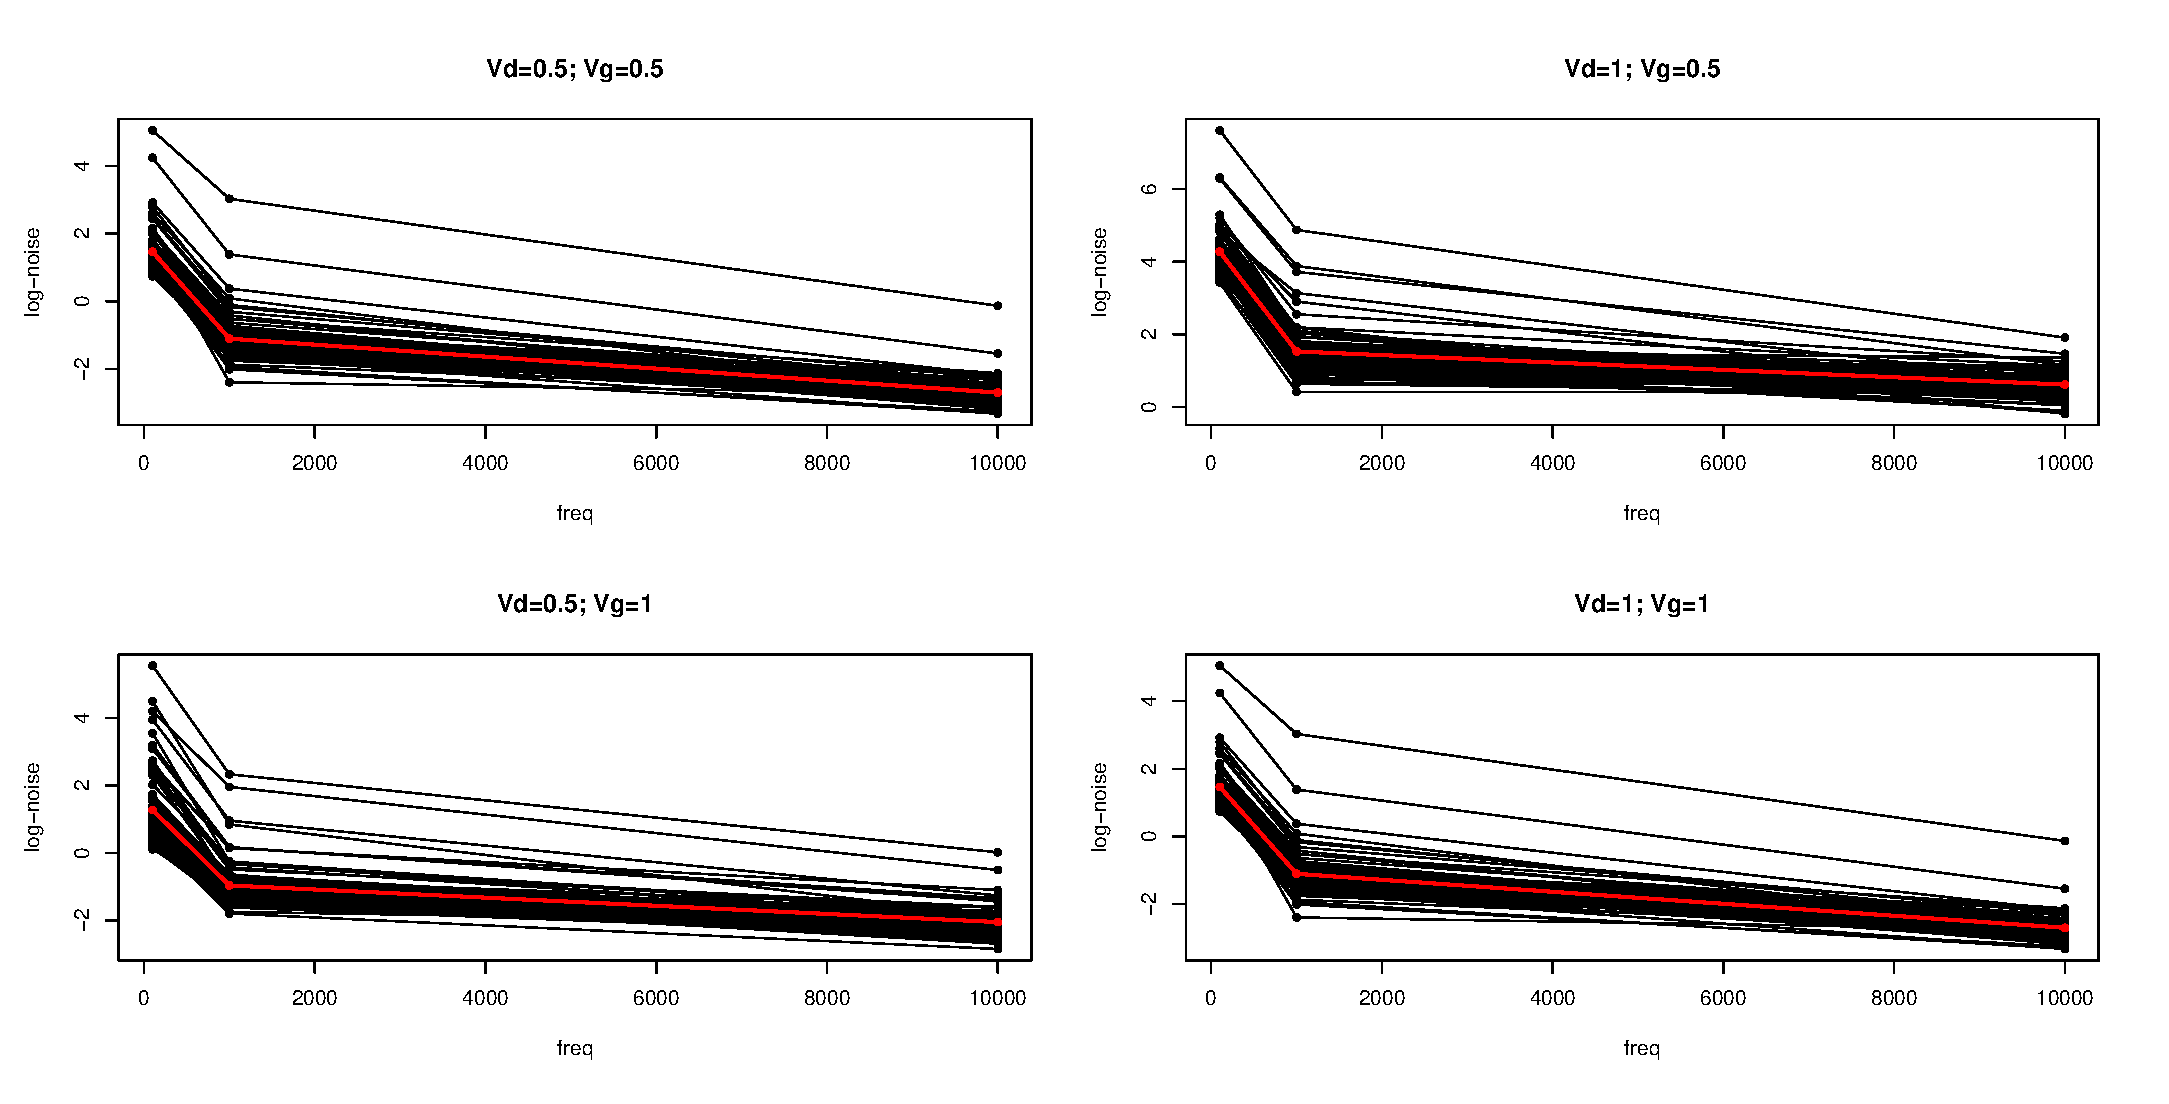
\includegraphics[width=0.4\textwidth]{Fig3_spaghetti.eps}}
	%\caption{Exploratory analysis: $Spaghetti$ diagram.}
	%\label{fig:spaghetti}
%\end{figure}
%%%%%%%%%%%%%%%%%%%%%%%%%%%%%%%%%%%%%%%%%%%%%%%%%%%%%%%%%%%%%%%%%%%%%%%%%%%%%%%%%%%%%%%%%%%%%%%%%%%%%%%%%%%%%%%%%%%%%%%%%%%%%%%%%%%%%%%%%%%%
\subsection{Linear regression models to predict 1/f Noise}
\label{sec:linear_model}
\noindent The simplest approach for predicting the value of $Noise$ given a set experimental conditions is to formulate a linear model with fixed effects for each $DIE$. Specifically, the value of $Noise_i$ (in $logarithmic$ scale) for the $i$-th sample unit, for $i=1,2,\ldots, 1068$, is expressed as 
\[
\log Noise_i  =\beta_0+\beta_{F1000}+\beta_{F10000} +\beta_{Vd1}+\beta_{Vg1}+\epsilon_i 
\]
where the intercept, $\beta_0$,  is the estimated $\log Noise$ for a $DIE$ measured at the baseline level of factors, that is $Freq$=100 Hz, $V_d=V_g=0.5$v. The rest of $\beta$-coefficients measure the relative change in $\log Noise$ scale when the corresponding covariate is considered at the levels indicated in the above expression.  For example, the coefficient $\beta_{F1000}$ quantifies the change in the response caused by changing the conditions from $Freq=100$Hz to $Freq=1000$Hz, controlling for the other factors, $V_d$ and $V_g$. The rest of coefficients in the model can be interpreted similarly.
The residual term $\epsilon_i$ represents the random error and it is assumed to be an independent realization of a random Normal variable  with mean 0 and standard deviation $\sigma$ (the same for all observations).\\

According to the above linear model, the change in $\log Noise$ caused by for example an increment of $Freq$ from 100 to 1000 is the same for all locations in the wafer. However we have seen in the previous inspection of the data, that we have reasons to believe that there are differences $between-subjects$ with respect to the effect that the covariates have on the variable $Noise$. In other words,  the variation of the value of $Noise$ when the level of $Freq$ is changed from 100 to 1000 is not constant along the different $DIE$s. On the contrary, there are random effects associated with the subjects ($DIE$s) that can modify the relationship factor-response from one location to another in the wafer. Therefore, the corresponding effect can take a specific value for each $DIE$, and the same conclusion is valid for the other factors $V_d$ and $V_g$.\\ 

To confirm these insights, we fit a linear model to each $DIE$-dataset. Specifically we fit a different linear model to explain the effect of each factor ($Freq$, $V_d$ and $V_g$) on the $\log Noise$ variation for each individual location on the wafer. One model  is built based on each $DIE$-dataset. This approach implies $89 \times 5=445$ parameters to be estimated. \\


The joint box-plot presented in Figure $\ref{fig:lm_coeff}$ corroborates some of the evidences suggested by Figure $\ref{fig:spaghetti}$. 
The $Intercept$ ($\beta_0$) represents the $\log Noise$ for the baseline level of covariates ($Freq=100$Hz, $V_d=0.5$v, $V_g=0.5$v).
%%%%%%%%%%%%%%%%%%%%%%%%%%%%%%%
\begin{figure}[ht]
	\centerline{
		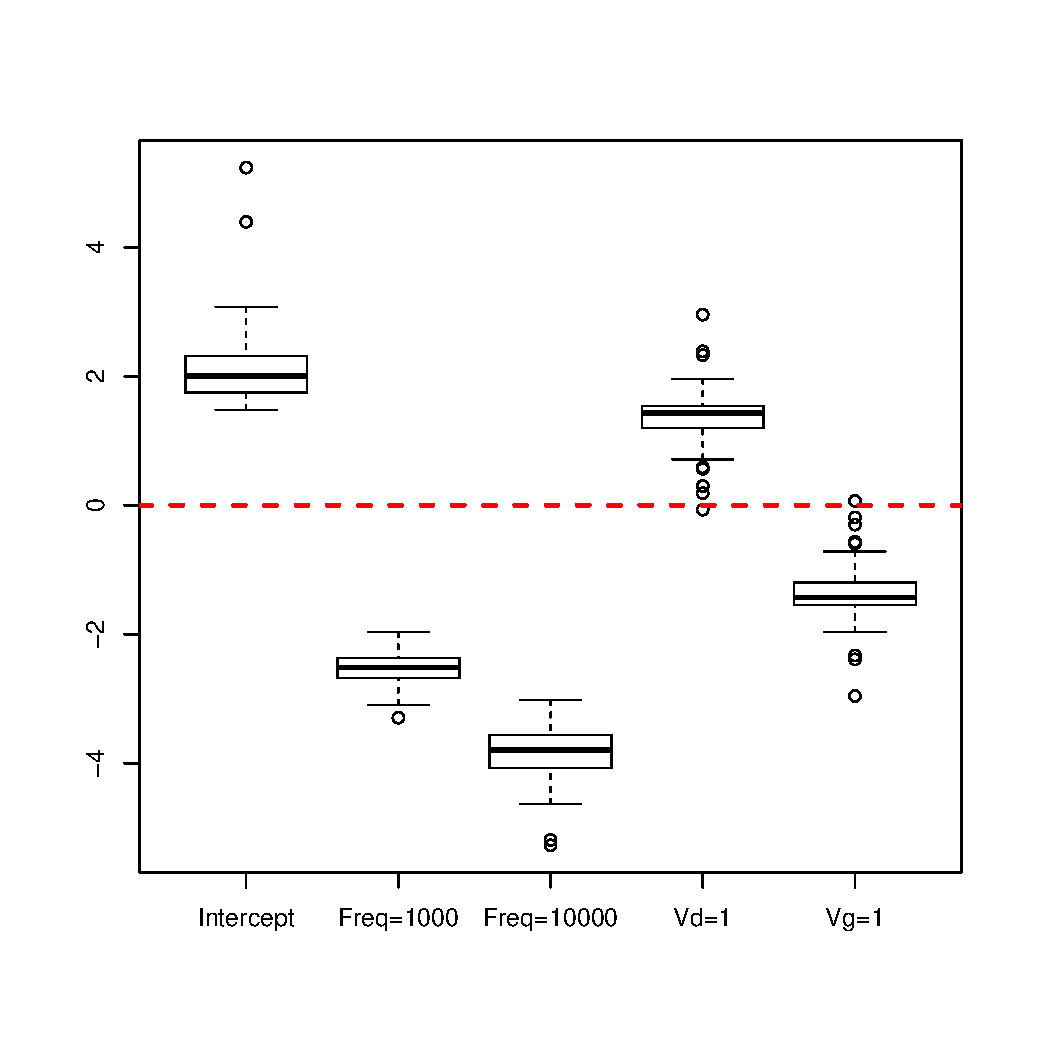
\includegraphics[width=0.6\textwidth]{Fig4_lm_coeff.eps}}
	\caption{Box-plot for coefficients of linear models along subjects.}
	\label{fig:lm_coeff}
\end{figure}

The remarkable variation exhibited by the values of some of the coefficients (in particular the intercept) suggests the existence of a random component associated to the subjects ($DIE$) that modifies the corresponding fixed effect. 
All the boxes (except the one for the factor $V_d$) lay on negative values, this means that in general, the $Noise$ is decreasing as the corresponding factor takes higher values. 
It is noticeable that the coefficients corresponding to $V_d$ and $V_g$ are near 0, which may be suggesting that these factors has smaller influence on the $Noise$ variable, in other words, changes in $V_d$ or $V_g$ will have little impact in $Noise$.




%%%%%%%%%%%%%%%%%%%%%%%%
%
\subsection{The repeated measures ANOVA model} \label{sec:anovaCheck}
\noindent From a statistical point of view, a model with 445 parameters is too complex to be useful and on the other hand, one important feature of the dataset is the underlying dependence structure  due to repeated measurements on each individual item. Then we can think of a repeated measures ANOVA model to fit the data. For the inference to be meaningful, the model must satisfy the assumption of normality of the residuals, and sphericity (i.e. the variance is constant for all differences between pairs of within-subjects measurements, see \cite{BHN2000}). When violations of the sphericity assumption occur in designs containing repeated measures, particularly when compounded by non-normality, as we will see it is the case in this study, the classical strategy for analysis is not entirely clear. As the sphericity assumption becomes more severely violated, the traditional unadjusted within-subjects F test is known to perform quite poorly, with its Type I error rate becoming extremely inflated (see \cite{BHN2000}).


To assess if the assumption of sphericity is met, we use the Mauchly's test of sphericity, together with the estimates of $\epsilon$, \cite{BHN2000}. From the results given in Table \ref{fig:mauchyls} we observe that all factors with more than two levels but the interaction between $Freq$ and $V_d$ show departures from sphericity. We confirm this by looking at the estimates of $\epsilon$ in Table \ref{tab:epsilontable}. 

\begin{table}[!t]
	\centering
	\caption{Mauchly's test of sphericity} 
	\begin{tabular}{lrr}
		\hline
		& $W$ &  $p$-value \\ 
		\hline
		$Freq$ & 0.719 & $<$ 0.001 \\ 
		$Freq \times V_d$ & 0.852   & $<$ 0.001 \\ 
		$Freq \times V_g$ & 0.852   & $<$ 0.001 \\ 
		$Freq \times V_d \times V_g$ & 0.909  & 0.016 \\ 
		\hline
	\end{tabular}
	\label{fig:mauchyls}
\end{table}


\begin{table}[!t]
	\centering
	\begin{tabular}{lrrrr}
		\hline
		& $\hat{\epsilon}$ & $p$-value &$\tilde{\epsilon}$&$p$-value \\ 
		\hline
		$ Freq$ & 0.781&$<$ 0.001  & 0.792 &$<$ 0.001 \\ 
		$Freq \times V_d$ & 0.871&$<$ 0.001  & 0.887&$<$ 0.001  \\ 
		$Freq \times V_g$ & 0.871&$<$ 0.001  & 0.887&$<$ 0.001  \\ 
		$Freq \times V_d \times V_g$ & 0.917&$<$ 0.001  & 0.935&$<$ 0.001  \\ 
		\hline
	\end{tabular}
	\caption{Estimates of $\epsilon$} 
	\label{tab:epsilontable}
\end{table}

Turning to the assumption of normality of the residuals, we deduce the quantile-quatile plot given in Figure \ref{fig:normalidad} that the residuals are non-normal, so the hypothesis of the model are not admissible. Having the above considerations into account, a repeated measures ANOVA model with Gaussian residuals is not appropriate to fit our data. 

%%%%%%%%%%%%%%%%%%%%%%%%%%%%%%
\begin{figure}[ht]
	\centerline{
		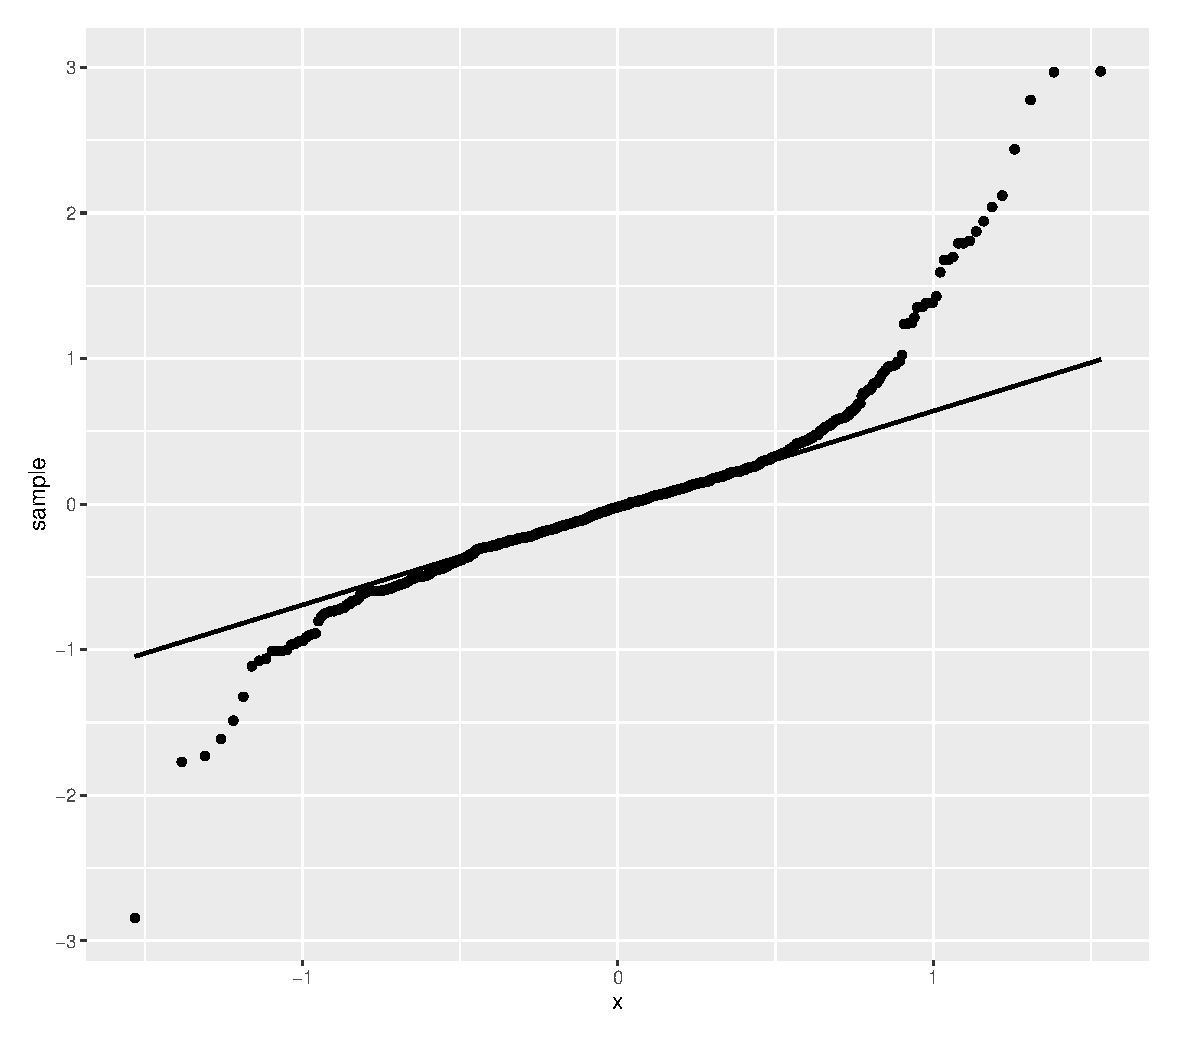
\includegraphics[width=0.6\textwidth]{Fig5_residuos.eps}}
	\caption{Quantile-quantile plot of residuals.}
	\label{fig:normalidad}
\end{figure}

%%%%%%%%%%%%%%%%%%%%%%%%
\subsection{The relationship 1/f noise $vs.$ threshold voltage, $V_{th}$} \label{sec:noiseVSvth}
The experimental study is mainly interested in evaluating the impact that the so called threshold voltage $V_{th}$ has on the 1/f noise. The threshold voltage is defined as the minimum gate-to-source voltage that is needed to create a conducting path between the source and drain terminals.\

As mentioned above, the threshold voltage values are extracted as explained in reference \cite{Duty2016}. It is expected that the values fit reasonably well a Gaussian distribution (see \cite{Duty2016} and \cite{Schroder2006}). However as we show in this section, the data do not support this usual assumption as can be deduced from the results provided by the tests of normality performed using the corresponding functions included in the software R, \cite{R2021}.


% latex table generated in R 4.1.0 by xtable 1.8-4 package
% Mon Jul 26 11:51:33 2021
\begin{table}[!t]
	\centering
	\begin{tabular}{|c|c|c|c|c|c|}
		\hline
		\multicolumn{3}{|c|}{Factors}&\multicolumn{2}{c|}{{\it Normality test ($p$-value)}} \\ \hline
		$Freq$ & $V_g$ & $V_d$ & $Pearson$ & $Shapiro-Wilk$ \\ 
		\hline
		100   & 0.5 & 0.5 & 0.0158 & 0.0000 \\ 
		&     & 1.0 & 0.0001 & 0.0000 \\ 
		& 1.0 & 0.5 & 0.0000 & 0.0000 \\ 
		&     & 1.0 & 0.0000 & 0.0000 \\ 
		1000  & 0.5 & 0.5 & 0.0058 & 0.0000 \\ 
		&     & 1.0 & 0.0000 & 0.0000 \\ 
		& 1.0 & 0.5 & 0.0000 & 0.0000 \\ 
		&     & 1.0 & 0.0000 & 0.0000 \\ 
		10000 & 0.5 & 0.5 & 0.8550 & 0.0019 \\ 
		&     & 1.0 & 0.8765 & 0.3678 \\ 
		& 1.0 & 0.5 & 0.0257 & 0.0000\\ 
		&     & 1.0 & 0.0174 & 0.0000\\ 
		\hline
	\end{tabular}
\end{table}

Besides, the same tests have been run with the $V_{th}$ observations and again the conclusion is that normality is not accepted based on this dataset, the corresponding $p$-values reported are  0.0022 for the Shapiro-Wilk test, and, 0.013, for the Pearson chi-square test.

Wrong conclusions can be drawn if we base on this hypothesis without corroborating it by means of the adequate statistic testing mechanisms.
For example, a parametric least-squares fit with normally distributed residuals would lead to the conclusion of absence of relation between $V_{th}$ and 1/f noise at all bias conditions considered here. However, a smoothed scatterplot obtained by means of locally-weighted polynomial regression, with no parametric restrictions for the variables involved, would lead to the plots presented in Figure \ref{fig:lognoiseVSvth}. We have represented a separate scatterplot for each combination of bias conditions and frequency. In total we have 12 fits. In absence of relationship, no tendency should be reflected by the fitted line to each scatterplot, which is not the situation for all cases. So we can not discard the existence of a relationship between $V_{th}$ and $Noise$ of some nature and then we need to explore this issue from a different perspective, where we build a model that also quantifies the effect of the different levels of the factor $Freq$ that have been considered in the design. Our proposal is presented in Section \ref{sec:model}.

%%%%%%%%%%%%%%%%%%%%%%%%%%%%%%%
\begin{figure}[ht]
	\centerline{
		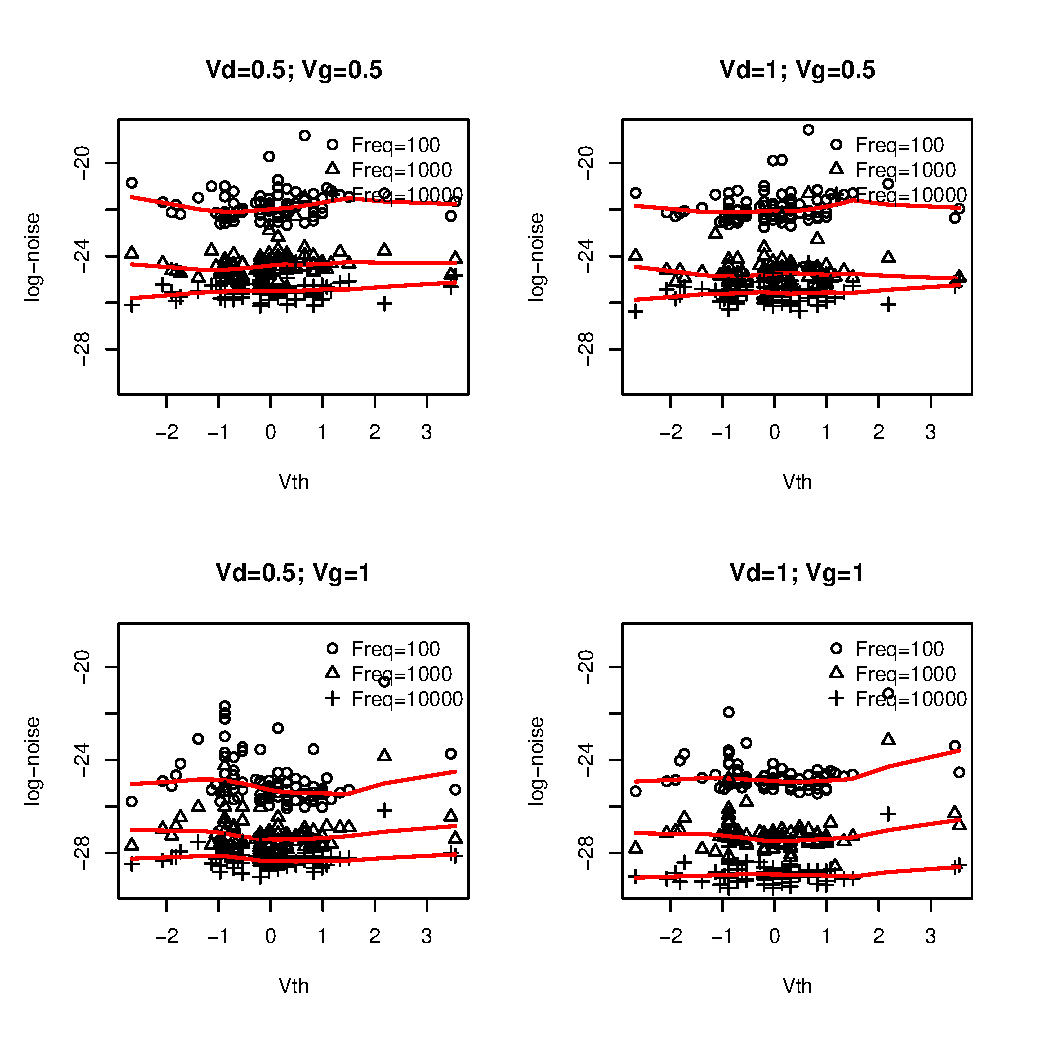
\includegraphics[width=0.7\textwidth]{Fig6_lognoiseVSvth.eps}}
	\caption{Smoothed scatterplot of $\log Noise$ vs. $V_{th}$ for different  bias conditions and frequency levels. }
	\label{fig:lognoiseVSvth}
\end{figure}



%\subsection{The spatial correlation issue}\label{sec:correlation}
%\noindent In this section  we  explore the  data focusing on the potential spatial auto-correlation induced by the experimental design that provided the dataset and that has been ignored so far.
%
%It is reasonable to assume that measurements associated to  adjacent cells are correlated and that the correlation decreases as the distance between cells increases. Therefore spatial autocorrelation should be in principle taken into account and then geo-statistical techniques are welcome. Figure \ref{fig:wafer} ({\it left panel}) presents the spatial arrangement of the units sampled in the grid (wafer). As explained in Section \ref{sec:dataset}, on the right panel of Figure \ref{fig:wafer} a pictorial representation of the values of $V_{th}$ measured on the wafer is given. The sample units are located at the cells labeled by proper $(x,y)$-coordinates. \
%
%\noindent The first step to study the spatial correlation is to estimate the variogram. In spatial statistics the theoretical variogram which is defined as ${\displaystyle 2\gamma ( {s} _{1},{s} _{2})}=Cov\left(Z(s_1),Z(s_2)\right)$ is a function describing the degree of spatial dependence of a spatial stochastic process ${\displaystyle Z({s} )} $. In our particular case, the stochastic process $Z(s)$ is determined by the 1/f noise variable (in logarithmic scale), measured for each spatial location given by $s$, at the different combinations of bias conditions and frequency levels. That is, the variable $s$ represents the  spatial location of a $DIE$ on the wafer and is expressed in terms of its $(x,y)$-coordinates in a regular 2-dimensional grid (wafer). The variogram thus gives a measure of how much two values of $log-Noise$ taken from the wafer at two different positions vary depending on the (Euclidean) distance between the two positions on the grid.
%The results for the bias conditions given by $V_d=0.5$v and $V_g=0.5$v are represented in Figure \ref{fig:varNoise1}. As can be appreciated the spatial autocorrelation is negligible for the considered levels of drain and gate voltage. \\
%In the following sections, the analytical procedures are developed considering only one type of dependency is present on the data: correlation induced by repeated measures.
%
%%%%%%%%%%%%%%%%%%%%%%%%%%%%%%%%
%\begin{center}
	%\begin{figure}[ht]
		%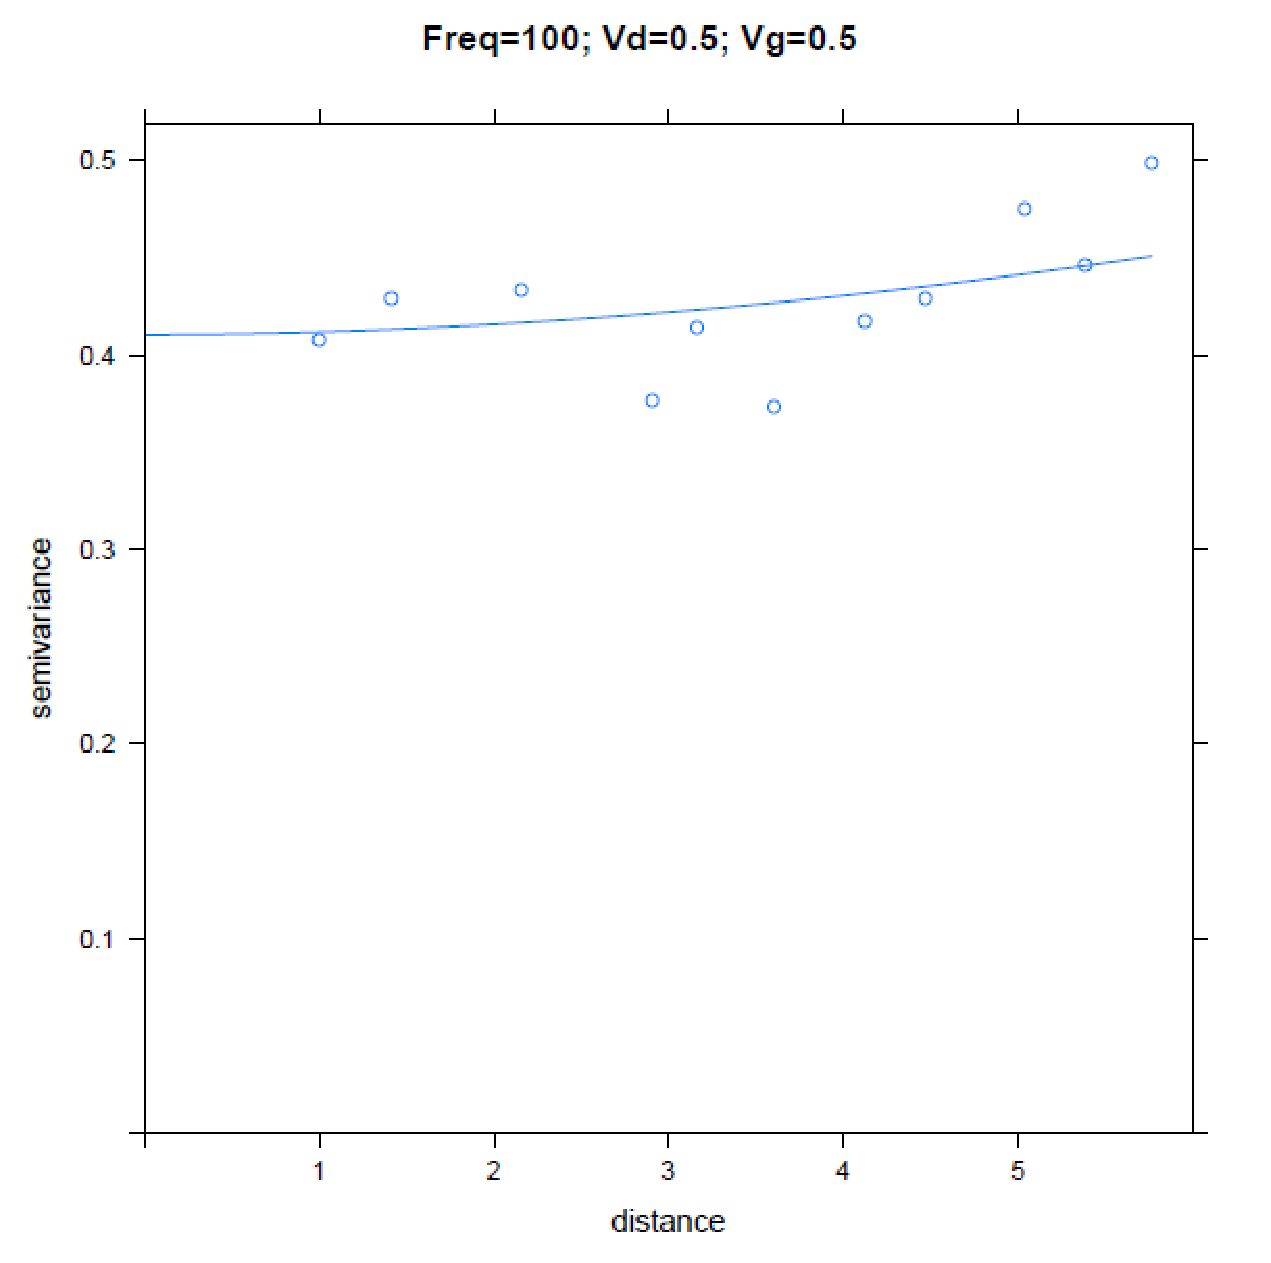
\includegraphics [width=0.3\textwidth]{Fig7_sheet11.eps} 
		%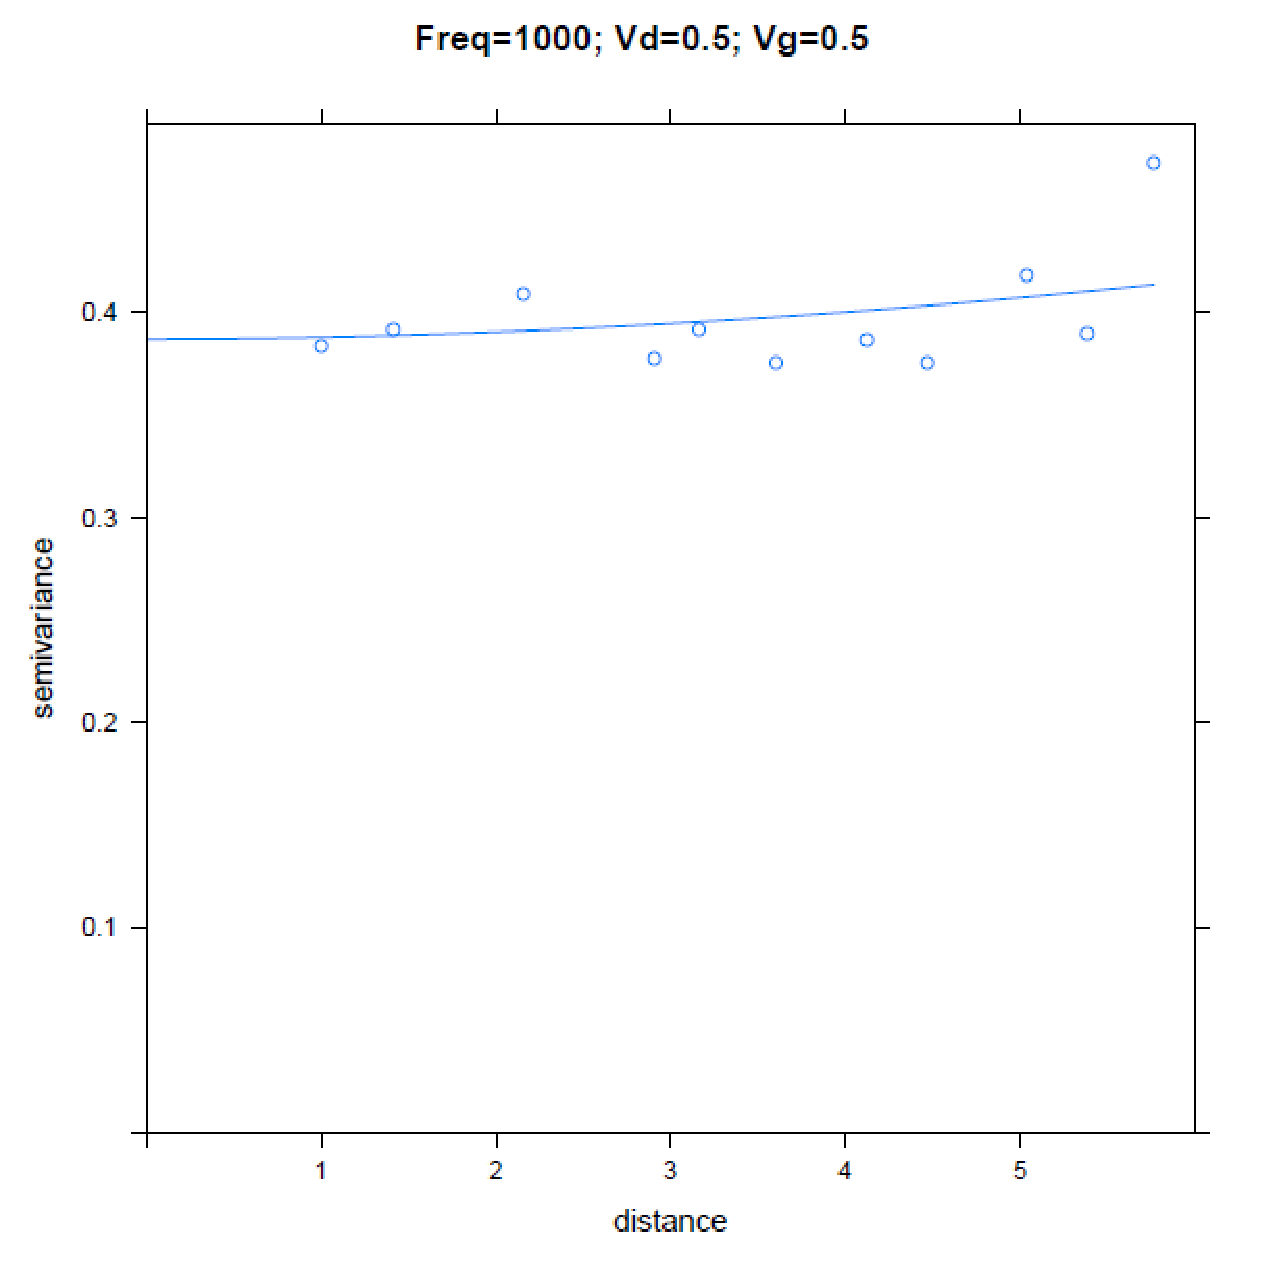
\includegraphics [width=0.3\textwidth]{Fig7_sheet12.eps}
		%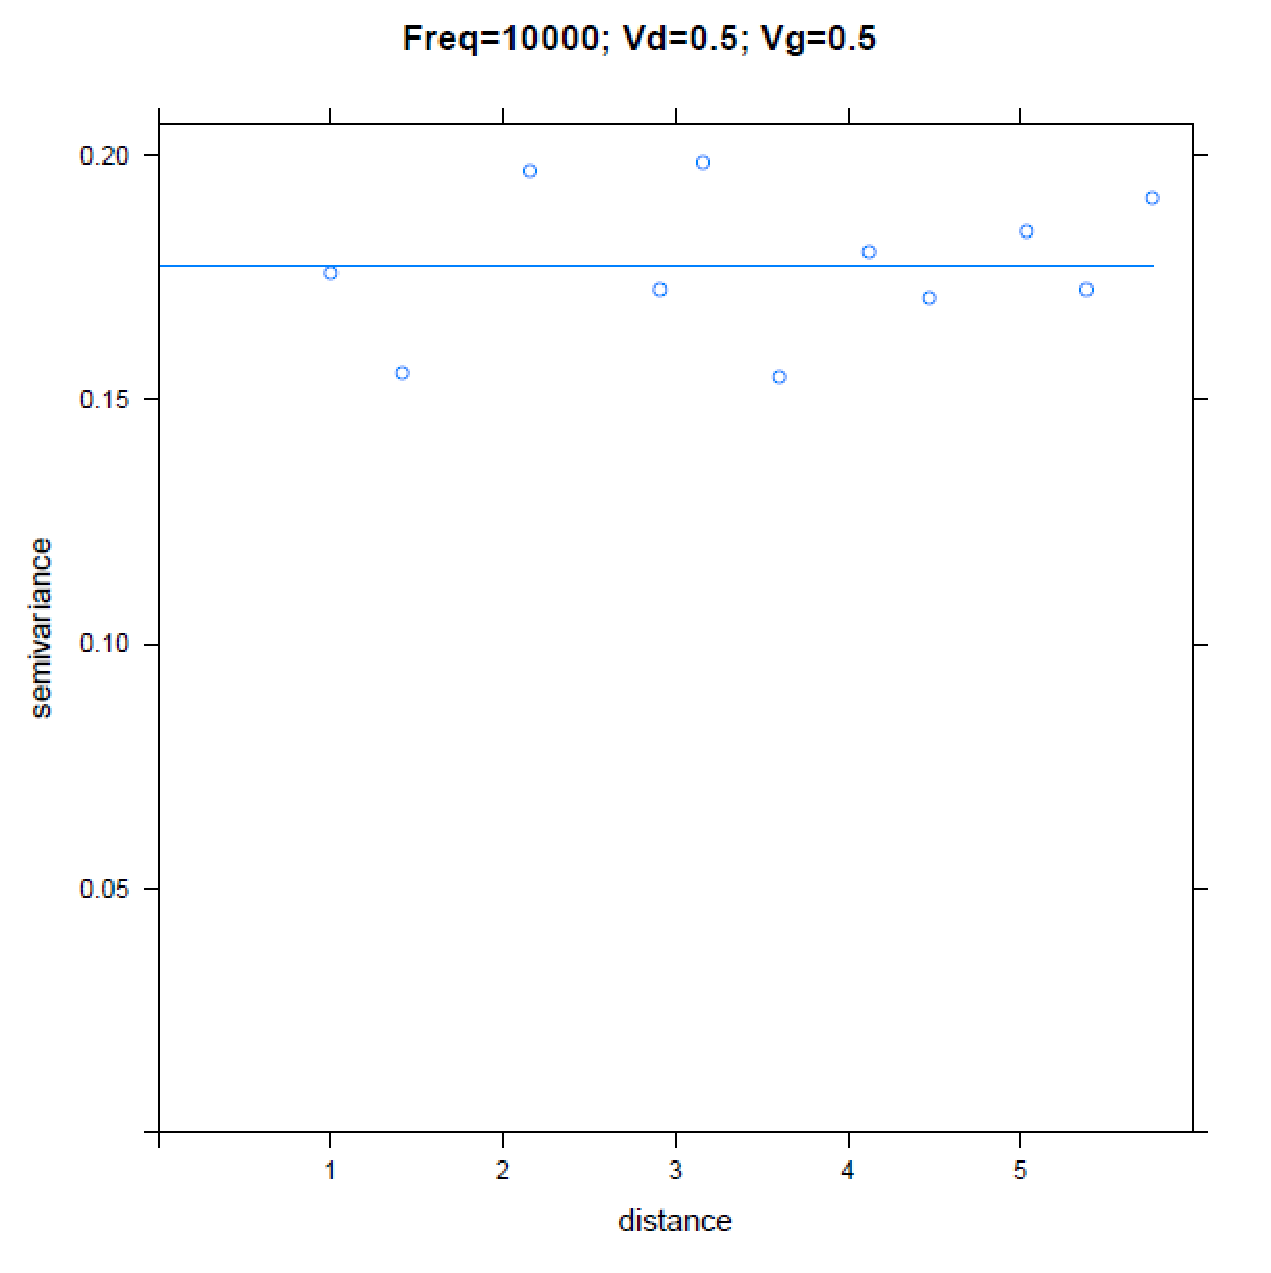
\includegraphics [width=0.3\textwidth]{Fig7_sheet13.eps}
		%\caption{Empirical variogram and power variogram model for $Noise$ random field (1).}
		%\label{fig:varNoise1}
	%\end{figure}
%\end{center}

%%%%%%%%%%%%%%%%%%%%%%%%%%%%%%%%%%%%%%%%%%%%%%%%%%%%%%%%%%%%%%%%%%%%%%%%%%%%%%%%%%%%%%%%%%%%%%%%%%%%%%%%%%%%%%%%%%%%%%%%%%%%%%%%%%%%%%%%%%%%
\section{The supervised learning algorithm proposed}\label{sec:model}

%A non-parametric three-factorial regression model with a random component}\label{sec:model} %\footnote{La correlacion espacial no esta ajustada de momento}

\noindent The data at hand come from a repeated measures design in which each experimental unit (e.g. $DIE$) is tested in more than one experimental condition, \cite{BHN2000}. In general, whereas observations on different units are assumed independent, the observations on the same subject are not. %Usually, the data from such experiments are analyzed through analysis of variance methods. 
%We have checked that the statistical assumptions for repeated measures ANOVA to be valid are not met in the practical application of this paper (results available). 
In this section we first discuss the proposed model and then we explain the algorithm to fit the data. Our method does not rely on strong parametric restrictions, on the contrary our method is data-driven. 
%
%, as it has been checked in the previous sections. A flexible approach for testing repeated measures main effect is the so-called {\it mixed-effects model analysis} which includes both fixed and random effects, see for example \cite{PB2000}. 
%The basic model is a linear model with random effects and errors normally distributed. 
%Motivated by the practical application, in our study we assume no particular distribution for both random effects and errors. We consider a semi-parametric formulation of the model  in the sense that a simple linear model may be adequate to describe subject-specific profiles in terms of random effects while the fixed effects are introduced in the model through an unspecified function.
%Moreover we must account for an extra feature: the spatial correlation structure underlying in the dataset. 

\subsection{The model}

\noindent We describe our proposal in a generic scenario although the main interest is the practical implementation  focused on the $DIE$ dataset described in Section \ref{sec:dataset}.\ %We do not consider interaction terms in our modelbecause it would increase the complexity of the model to such an extend that the result would not be easily interpretable being not useful for our purpose. \\
Let us consider 
\begin{equation} \label{eq:mix_model}
	y_{ij} = m(x_i)+ b_{j}+\gamma_{i}+ \epsilon_{ij};
\end{equation}
where 
\begin{itemize}
\item $y_{ij}$ are the observed responses that are related to a one-dimensional numeric covariate $X$ and a factor $Z$ with levels $Z_j$, $j=1,2,\ldots, J$. For a specific subject $i$ the value  $X=x_i$ is observed, and the response is measured for all subjects at all levels of factor $Z$, then, $y_{ij}$ is the response of subject $i$ when tested at level $Z_j$, $i=1,2,\ldots, n$; $j=1,2,\ldots, J$;

\item $m(\cdot)$ represents the fixed effect or population function. It quantifies the relationship between the response and the covariate, and it is assumed not to change across the levels of $Z$. No specific functional form for $m$ is considered, the only assumption is that it is a smooth function in the sense of derivability. 

\item $b_j$ is the fixed effect coefficient of level $Z_j$, $j=1, \ldots, J$. The restriction $\sum_{j=1}^J b_j=0$, must be met for identifiability of the model.

\item $\gamma_i$  is the random effect associated to the $i$-th subject. For two different subjects, $i \neq i'$, $\gamma_i$ y $\gamma_{i'}$ are random variables with mean 0 and variance  $\sigma_{\gamma}^2$. We assume this variable is specific to the  subject $i$ and it is not related to the particular combination of levels of the factors the subject is tested at. 


\item $\epsilon_{ij}$ is the component of random error or residual. It is associated to the subject $i$ and also to the level $Z_j$. They are assumed to be independent random variables identically distributed with mean 0. %\footnote{ In the classic model the residuals are assumed to be incorrelated random variables with  $N(0, \sigma_e^2)$ distribution}. 
Moreover, for all $i$ and $j\neq j'$, it is assumed that $Cov(\epsilon_{ij},\epsilon_{ij'})\neq 0$.
\end{itemize}


%%%%%%%%%%%%%%%%%%%%
\bigskip
We assume that $m$ is two times continuously differentiable. Then for any fixed $x$ in a generic domain $\mathcal{X}$, $m$ can be approximated by a linear function within a neighborhood of $x$ by a Taylor expansion, i.e.
$$m(x_i)\approx \beta_0 +\beta_1(x_i-x)$$
where we denote $\beta_0=m(x)$ and $\beta_1=m'(x)$. Setting ${\bf x}_i=\left(1,x_i-x\right)^t$ model \eqref{eq:mix_model} can be approximated by the local linear mixed effects model
\begin{equation}\label{eq:LLme}
y_{ij} = {\bf x}_i \bbeta + b_j+ \gamma_i + \epsilon_{ij}
\end{equation}
for all $x_i$ sufficiently near $x$, that is $|x_i-x|<h$, for $h$ small enough. The parameter $h$ that controls the size of the interval around $x$  where the linear approximation is valid is called the bandwidth parameter. 

%%%%%%%%%% Relacion con otros trabajos:

%% Wu \& Liang (2004):
In this paper we propose a backfitting algorithm to estimate the model formulated in \eqref{eq:LLme}. 
The classical backfitting technique was introduced by \cite{BHT1989} and later in \cite{HT1990} to estimate additive models. It has proven good performance through simulations as well as applications to real data problems and a complete theory  for the two-dimensional model can be found in \cite{OR1997} and \cite{Opsomer2000} extended to high dimensional problems. \cite{WL2004} proposed  a backfitting algorithm to fit a random-varying coefficient model based on longitudinal data. They used similar ideas to mixed-effect model to account for time-varying effects as well as intra-subject dependence structure. The real dataset we are analyzing can be seen as a longitudinal study with the frequency-domain playing the role of time-domain of a typical longitudinal study.  Our model is close to the model proposed in \cite{WL2004}, with important discrepancies. In our case the covariate ($V_{th}$) is not a longitudinal variable, so that  the effect of the covariate on the response do not vary with frequency. On the other hand, unlike the work of \cite{WL2004}, the covariate is introduced in the model fully non-parametrically. We sketch in the following the steps of our algorithm.


\subsection{Backfitting algorithm}\label{sec:backfit}

Let us denote $\bar{y}_{\cdot j} =n^{-1}\sum_{i=1}^n y_{ij}$, for all $j=1, 2,\ldots, J$; $\bar{y}_{ i \cdot} =J^{-1}\sum_{j=1}^J y_{ij}$, for all $i=1,2,\ldots, n$; and, $\bar{y}_{\cdot \cdot} =(n  J)^{-1}\sum_{i=1}^n \sum_{j=1}^J y_{ij}$.\

\subsubsection*{ Algorithm 1}
\begin{enumerate}
\item[Step 1.] \textit{Initialization}. \\
 \noindent Set $r=0$ and define
$$b_j^{(r)}=\bar{y}_{\cdot j}-\bar{y}_{\cdot \cdot};$$
$$\gamma_i^{(r)}=\bar{y}_{i \cdot}-\bar{y}_{\cdot \cdot};\ {\rm and}, $$
$$m^{(r)}(x_i)=0.$$ 

\item[Step 2.]  \textit{Smoothing}.\\
\noindent Put $r=r+1$, and define $y_{ij}^{(r)}=y_{ij}-b_j^{(r-1)}-\gamma_i^{(r-1)}$, for all $i=1, \ldots, n$ and $j=1,2,3$.

Then, estimate $m(x)$ locally by kernel smoothing. That is, for fixed $x_0 \in \mathcal{X}$, find ${\beta}^{(r)}_0={m}^{(r)}(x_0)$; and, ${\beta}^{(r)}_1={m'}^{(r)}(x_0)$ as the minimizers of the following expression

\begin{equation*}
%&&\left({\beta}^{(r)}_0, {\beta}^{(r)}_1 \right)^t \\
%\displaystyle{\underset{({\beta}_0,{\beta}_1)}{\arg \min} \ 
\sum_{i=1}^n\sum_{j=1}^J\left\{y_{ij}^{(r)}-\beta_0-\beta_1(x_i-x_0)\right\}^2 \ K_h\left(x_i-x_0\right)%}
\end{equation*} 
where $K_h(\cdot)=K(\cdot/h)/h$, with $K(\cdot)$ a kernel function. \


\item[Step 3.] \textit{Mixed-effects model fitting}. \\
\noindent Put $r=r+1$, and define $y_{ij}^{(r)}=y_{ij}-{m}^{(r-1)}(x_i)$, for all $i=1, \ldots, n$ and $j=1,2,3$. 
Then fit the following mixed-effects model:
\[
y_{ij}^{(r)}= b_j +\gamma_i + \epsilon_{ij}, \hspace{0.5cm} i=1, \ldots, n; \ j=1,2,3;
\]
or, in matrix notation,
\[
{\bf y}_{i}^{(r)} = {\bf b} +\gamma_i + {\boldsymbol \epsilon}_i
\]
where ${\bf b}=(b_1,b_2,b_3)^t$, is a vector of fixed effects, and $\gamma_i$ is a random effect such that $\gamma_i \sim (0, \sigma_{\gamma})$, and the residuals ${\boldsymbol \epsilon}_{i} \sim (0,{\mathbf \Sigma}_i)$, with ${\mathbf \Sigma}_i$ a covariance matrix of dimension $J \times J$. Then, suitable estimations can be obtained by minimizing the following objective function (see \cite{DG2003})
\[
\sum_{i=1}^n \left\{ ({\bf y}_i-{\bf b}-\gamma_i) {\mathbf \Sigma}_i^{-1}({\bf y}_i-{\bf b}-\gamma_i)+ \gamma_i^2/\sigma_{\gamma}^2\right\}.
\]
Since $\sigma_{\gamma}$ and ${\mathbf \Sigma}_{i}$ are unknown, to solve the minimization problem we use linear mixed model software such as function ${\rm lme} ()$, see \cite{PB2000}. We extract the 
 best linear unbiased predictions (BLUPs) of the random effects from the fitted model, which are denoted $\gamma_{i}^{(r)}$ for $i=1, 2, \ldots, n$, as well as the estimations of the fixed effects, denoted as $b_{j}^{(r)}$, $j=1,2,\ldots, J$. 
%\\
  %$$b_j^{(r)}=\frac{1}{n}\sum_{i=1}^n\left(y_{ij}-{m}^{(r)}(x_i)\right)=\bar y_{\cdot j}-\bar{m}^{(r)};\ {\rm and},$$
%$$\gamma_i^{(r)}=\frac{1}{J}\sum_{j=1}^J\left(y_{ij}-{m}^{(r)}(x_i)\right)=\bar y_{i\cdot }-{m}^{(r)}(x_i);$$
%where $\bar{m}^{(r)}=\frac{1}{n}\sum_{i=1}^n {m}^{(r)}(x_i)$.

\item[Step 4.] \textit{Convergence}. \\
\noindent Repeat Steps 2-3 until convergence, that is, until the difference between two consecutive estimations is small enough. More specifically, stop at the $r$-th iteration when
{\small{
\[
\frac{\displaystyle{\sum_{i=1}^n} \left(\widehat{m}^{(r)}(x_i)-\widehat{m}^{(r-1)}(x_i)\right)^2}{\displaystyle{\sum_{i=1}^n}\widehat{m}^{(r-1)}(x_i)^2+10^{-4}}<10^{-4}
\]
}}
\end{enumerate}

\subsection{Some theory}
\subsubsection{Asymptotic properties of the nonparametric estimator, $\widehat{m}$}
Given the specifications of our model, the solution of the local-linear smoothing problem settled in the Step 2 (smoothing) of the algorithm is the same as the solution of the following problem. Find $\widehat{\beta}_0$; and, $\widehat{\beta}_1$ as the minimizers of the following expression
 \[
 \sum_{i=1}^n\left\{\bar{y}_{i\cdot}-\beta_0-\beta_1(x_i-x_0)\right\}^2 \ K_h\left(x_i-x_0\right),%},
 \]
where, as defined above  $\bar{y}_{i \cdot} =J^{-1}\sum_{j=1}^Jy_{ij}$. 

Now we can appeal to the theory on nonparametric estimation given in \cite{FG1996} to establish the asymptotic properties of the estimator obtained. In particular, we can obtain a limit (asymptotic)  expression of the mean squared error, that is, $MSE(x)=E\left[\widehat{m}_h(x)-m(x)\right]$, as follows. 

Let $f(x)$ denote the density function of the covariate $X$; $m''(x)$ is the second derivative of the function $m$. Associated to the kernel function $K$, let us define the following: $R(K)=\int K^2(u)du$; and, $\mu_2=\int u^2K(u)du$. And finally, denote ${\bf u}$ the column vector of dimension $J$ with all its components equal to 1. Then, when $n \rightarrow +\infty$, the asymptotic MSE is given by
\begin{equation*}
AMSE(\widehat{m}_h(x))=\frac{h^4}{4}m''(x)^2\mu_2^2(K)+\frac{1}{nh}\frac{{\bf u}^t { \Sigma} {\bf u}}{f(x)}R(K)+o(h^4+(nh)^{-1})
\end{equation*}
where $o(\cdot)$ is function with the property $o(t)/t \rightarrow 0$, when $t \rightarrow 0$. From this expression we can deduce the consistency of the estimator, which means that the estimator is closer to the true function as $n \rightarrow +\infty$. 
The first term of the sum gives the asymptotic bias of the estimator, while the second one gives the asymptotic variance. As can be seen the choice of the bandwidth parameter is important to keep the balance between the two terms. A bandwidth $h \approx n^{-1/5}$ will lead to asymptotic bias and variance of the same order, and then the asymptotic error of the estimator is of order $o(n^{-4/5})$. 

\subsubsection{The bandwidth parameter, $h$}
One problem inherent to kernel smoothing is the appropriate choice of the bandwidth or smoothing parameter $h$. 
The literature on the subject is very extensive and various methods compete when choosing the value of the parameter that provides the resulting estimator with the optimal properties (see for example \cite{FG1996} for details). The selection of the bandwidth in our context will not be treated in this paper. For the examples that will be seen below, different options have been tested leading to similar results. Finally to estimate the curves presented in the Figures \ref{fig:backfit1}-\ref{fig:backfit2} corresponding to the real application, as well as for estimated curves of Figure \ref{fig:estim_m} in the simulations, plug-in bandwidth selection has been considered.

To avoid potential, and not desirable, influence of the bandwidth, in Section \ref{sec:sizer} we use a multiscale methodology to solve the contrast problem formulated there. This methodology allows solving the problem without being conditioned by any concrete bandwidth.

\section{Numerical results}\label{sec:result}

\subsection{Real dataset}\label{sec:bf_noise}

In this section we apply the backfitting algorithm defined in \ref{sec:backfit} to the dataset consisting of noise measurements observed on a wafer as  described in Section \ref{sec:dataset}. As explained previously, the wafer is divided in $n=89$ $DIE$s and each one has been tested four combinations of gate voltage and drain voltage, and three different levels of frequency. 
The variable response is the noise measured on the DIE in logarithmic scale, $Y$. We have considered the data for each combination of drain voltage ($V_d$) and gate voltage ($V_g$), so we have 4 different sub-samples of size $267$ each. We have run the algorithm separately for each sub-sample and the results obtained for all cases have been compared. 
  It is supposed that the response $Y$ depends on one covariate $X=V_{th}$, and one factor $Z=Frequency$. Besides, we consider a random term in the model specified by each particular subject or $DIE$.

The semi-parametric mixed-effects model of equation \eqref{eq:mix_model} has been fitted to the data separately for the four sub-samples that are determined by the different bias conditions: $V_d=V_g=0.5$v (Figure \ref{fig:backfit1}),  $V_d=1$, $V_g=0.5$v (Figure \ref{fig:backfit2}), $V_d=0.5$v, $V_g=1$v (Figure \ref{fig:backfit3}), $V_d=1$v, $V_g=1$v (Figure \ref{fig:backfit4}). The estimations of the parameters involved in the model are given in Table \ref{tab:estim_noise}. In concrete, columns 1-3 give the estimated components of the fixed-effect parameter vector due to the different levels of the factor $Z$; and, column 4 gives the estimation of the standard deviation of the random-effect induced by the different $DIE$s, that is $\sigma_{\gamma}$.
\begin{table}[!t]
	\begin{center}
		\caption{Semi-parametric mixed-effects model for 1/f noise dataset}
		\label{tab:estim_noise}
		\begin{tabular}{|c|c|c|c|c|} \hline
			%\multicolumn{1}{c}{}&\multicolumn{3}{c}{Fixed effects}&\multicolumn{1}{c}{Random effect}\\ \hline
			Bias conditions     &$b_{100Hz}$  &$b_{1000Hz}$   &$b_{10000Hz}$     &$ \sigma_{\gamma}$ \\ \hline
			$V_d=V_g=0.5$v       &1.854  &-0.667 	&-1.781 	 &  0.295  \\ \hline
			$V_d=1$v; $V_g=0.5$v &1.019	 &-1.218  &-2.305 	 &  0.553 \\ \hline
			$V_d=0.5$v; $V_g=1$v &2.282  &-0.464  &-1.384	   &  0.376  \\ \hline
			$V_d=V_g=1$v         &1.643	 &-0.925  &-2.5194	 &  0.437  \\ \hline
		\end{tabular}
	\end{center}
\end{table}


The results regarding the nonparametric component of the mixed model are displayed in Figures \ref{fig:backfit1}-\ref{fig:backfit4}, where it is represented the final estimation of the function $m(x)$ for all the four samples obtained at different bias conditions. Figure \ref{fig:backfit1}, displays the fixed effect function $m$  fitted plus the corresponding fixed effect due to each level of the factor $Z=Frequency$, i.e. ${\bf b}$. From left to right, it is represented, for each value of the covariate $V_{th}$, the estimated value of the nonparametric component plus the corresponding estimation of the $b_j$ coefficient, for $j=1,2, 3$. The left panel represents, in all Figures \ref{fig:backfit1}-\ref{fig:backfit4}, the obtained estimation for $Z=100$Hz; the middle panel gives the result for $Z=1000$Hz; and, the right panel gives the result for $Z=10000$Hz.  As can be appreciated from the estimations in Table \ref{tab:estim_noise}, and the corresponding figures when the $DIE$s are working under gate voltage $V_g=1$v, the measured noise values increase as well as the variability. Also the estimated nonparametric component, which controls the effect of the threshold voltage on the noise reported presents certain curvature indicating a change of trend. In particular, in Figure \ref{fig:backfit4} that displays the results for the $DIE$s working at a drain voltage $V_d=1$v, the curve seems to describe an increasing tendency, meaning that the higher the switching threshold voltage  the higher noise power level produced by the signal. In Section \ref{sec:sizer} below we discuss this question more in depth.
%%%%%%%%%%%%%%%%%%%%%%%%%%%%%%

\begin{figure}[ht]
	\centerline{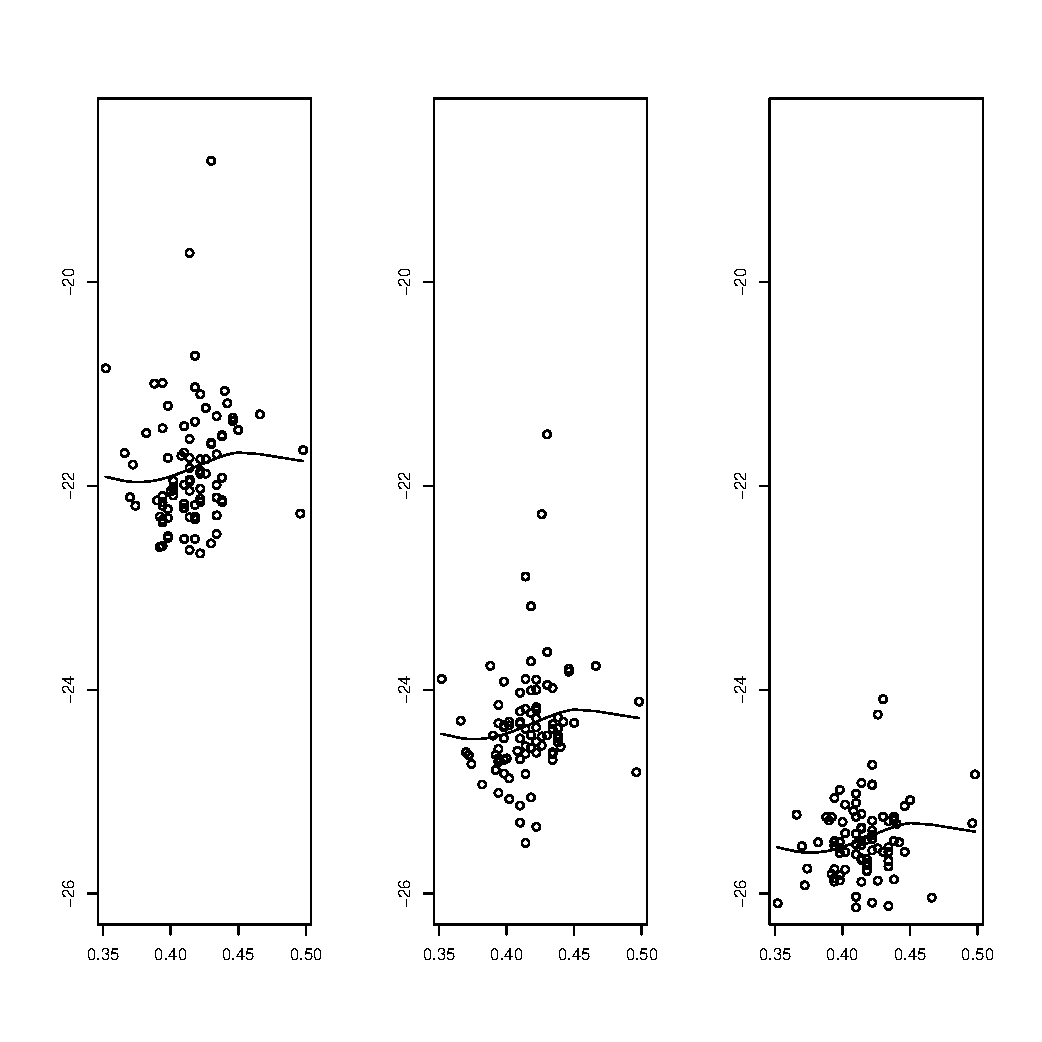
\includegraphics [width=0.6\textwidth]{Fig8_elognoise_d05g05.eps}}%{backfit_g1.eps} }
	\caption{Estimation of the nonparametric component $m(x)$ of the mixed-effects model \eqref{eq:mix_model}, using the backfitting algorithm for data of 1/f noise measurements obtained under bias conditions $V_d=0.5$v and $V_g=0.5$v, and for all $Freq$ levels. In panels from left to right: 100Hz, 1000Hz and 10000Hz, respectively.}
	\label{fig:backfit1}
\end{figure}
\begin{figure}[ht]
	\centerline{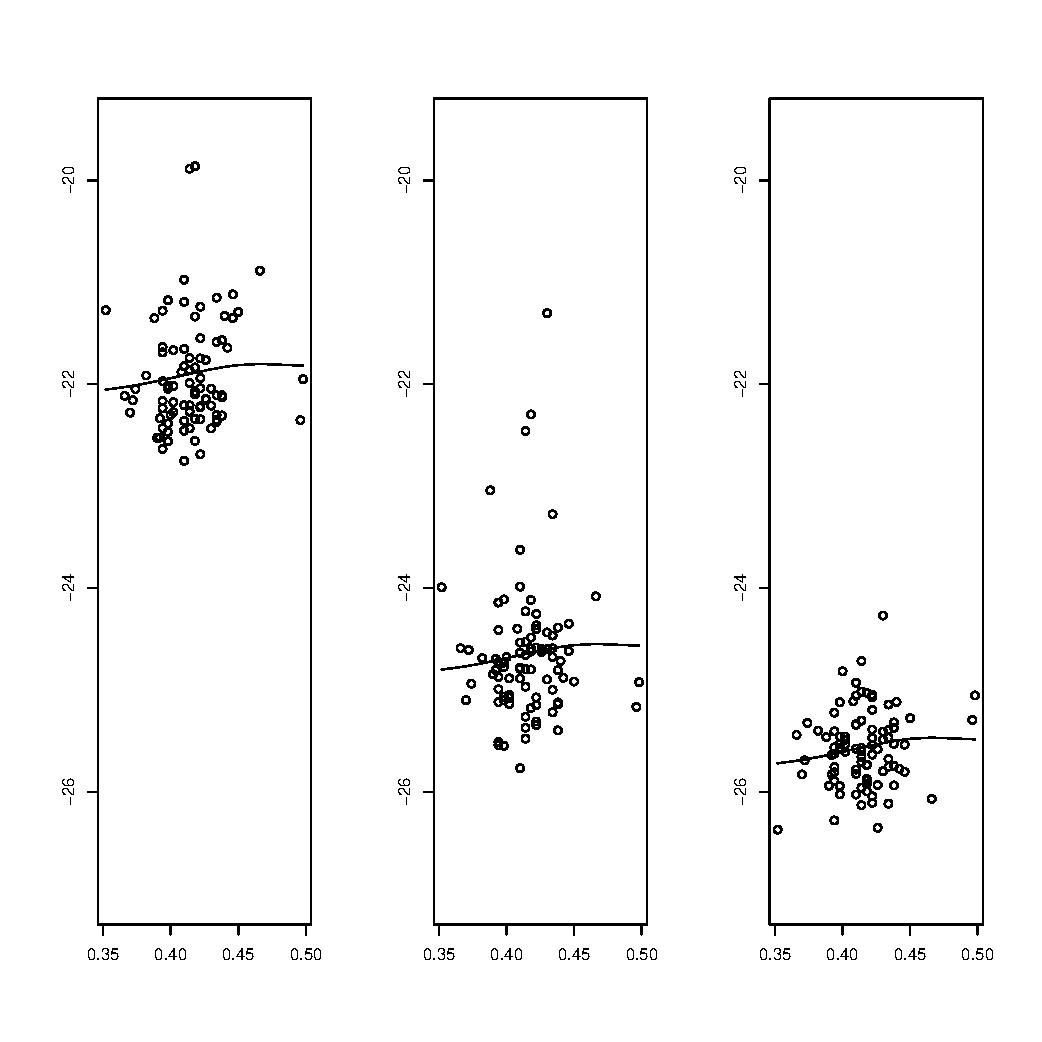
\includegraphics [width=0.6\textwidth]{Fig9_elognoise_d1g05.eps}}%backfit_g2.eps} }
	\caption{Estimation of the nonparametric component $m(x)$ of the mixed-effects model \eqref{eq:mix_model}, using the backfitting algorithm for data of 1/f noise measurements obtained under bias conditions $V_d=1$v and $V_g=0.5$v, and for all $Freq$ levels. In panels from left to right: 100Hz, 1000Hz and 10000Hz, respectively.}
	\label{fig:backfit2}
\end{figure}
\begin{figure}[ht]
	\centerline{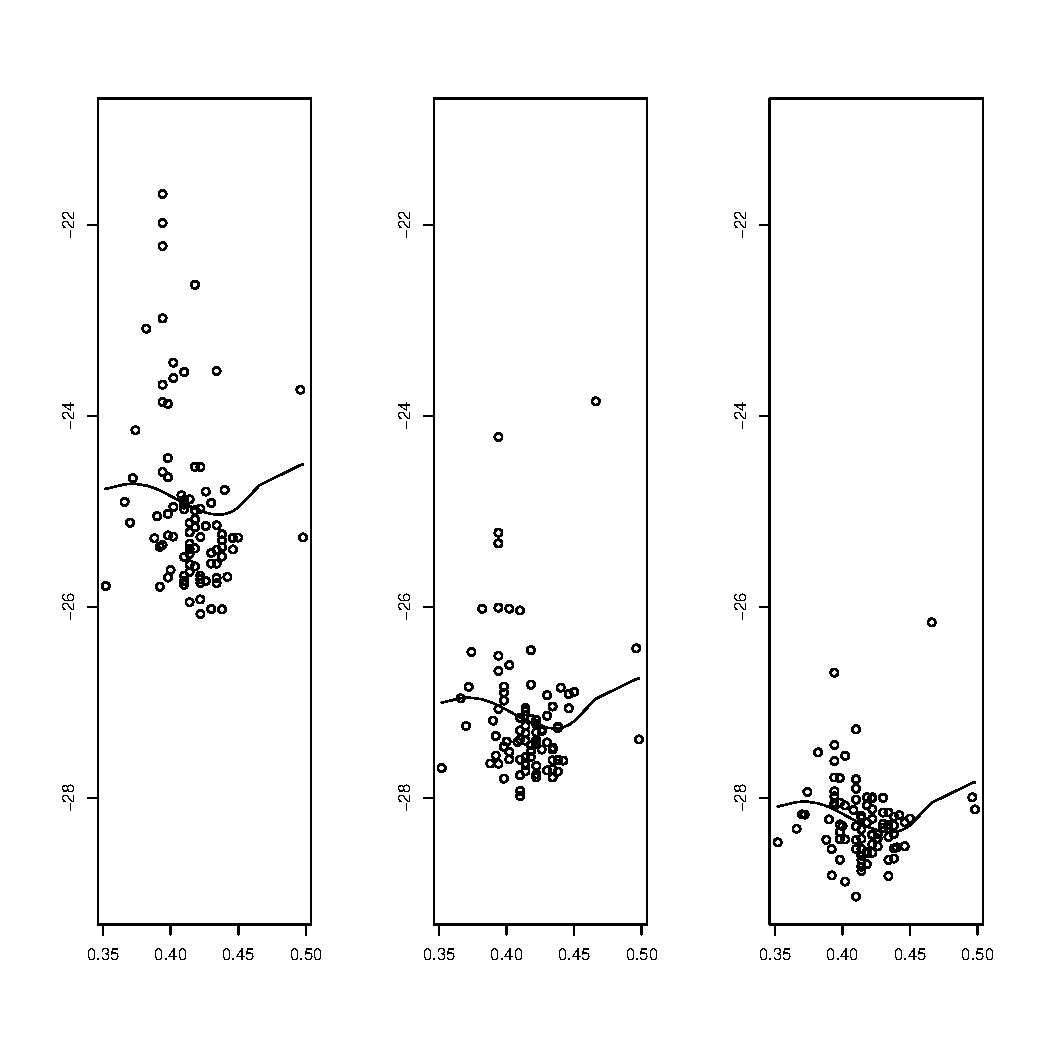
\includegraphics [width=0.6\textwidth]{Fig10_elognoise_d05g1.eps}}%{backfit_g3.eps} }
	\caption{Estimation of the nonparametric component $m(x)$ of the mixed-effects model \eqref{eq:mix_model}, using the backfitting algorithm for data of 1/f noise measurements obtained under bias conditions $V_d=0.5$v and $V_g=1$v, and for all $Freq$ levels. In panels from left to right: 100Hz, 1000Hz and 10000Hz, respectively.}
	\label{fig:backfit3}
\end{figure}
\begin{figure}[ht]
	\centerline{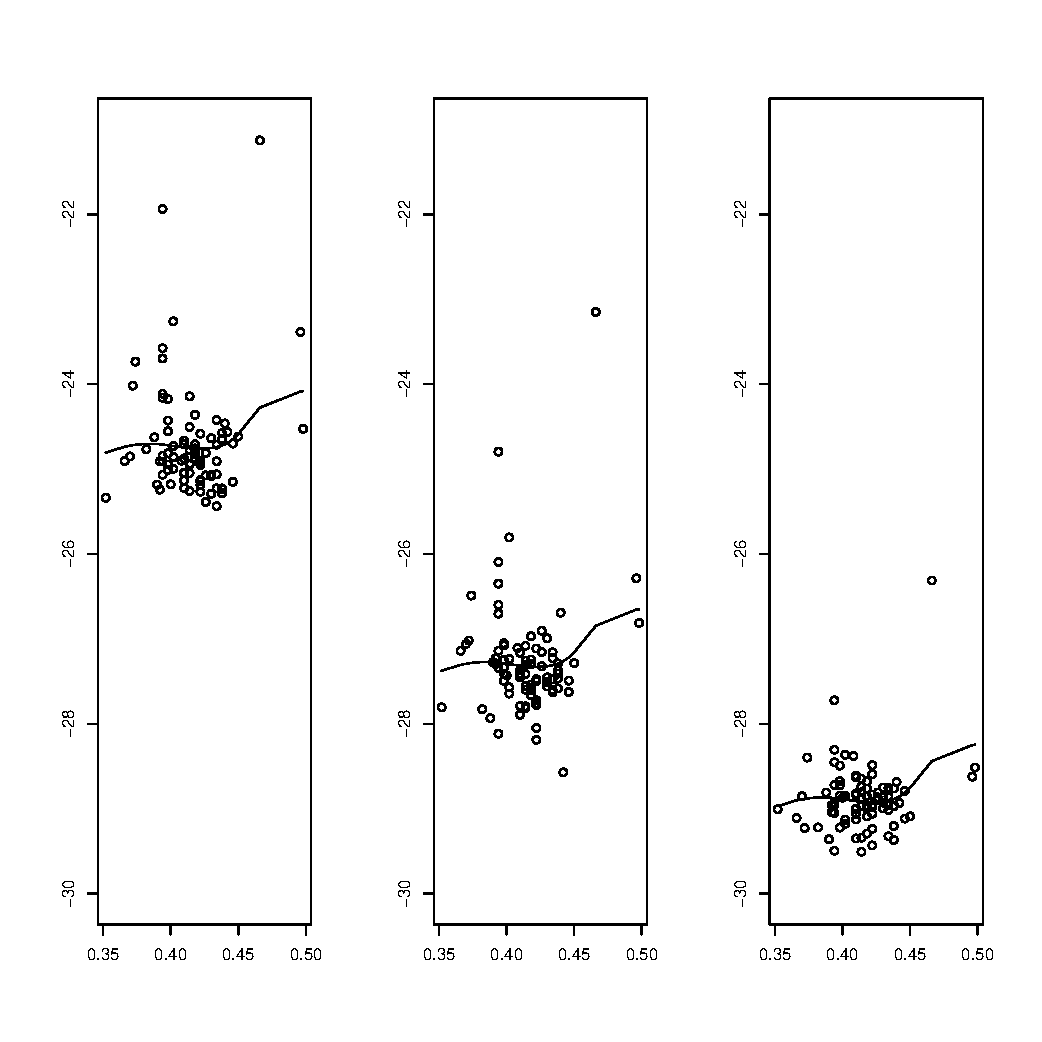
\includegraphics [width=0.6\textwidth]{Fig11_elognoise_d1g1.eps}}%{backfit_g4.eps} }
	\caption{Estimation of the nonparametric component $m(x)$ of the mixed-effects model \eqref{eq:mix_model}, using the backfitting algorithm for data of 1/f noise measurements obtained under bias conditions $V_d=1$v and $V_g=1$v, and for all $Freq$ levels. In panels from left to right: 100Hz, 1000Hz and 10000Hz, respectively.}
	\label{fig:backfit4}
\end{figure}

%%%%%%%%%%%%%%%%%%%%%%%%%%%%%%%%%%%%%%%%%%%%%%%%%%%%%%%%%%%%%%%%%%%%%%%%%%%%%%%%%%%%%%%%%%%%%%%%%%%%%%%%%%%%%%%%%%%%%%%%%%%%%%%%%%%%%%%
%%%%%%%%%%%%%%%%%%%%%%%%%%%%%%%%%%%%%%%%%%%%%%%%%%%%%%%%%%%%%%%%%%%%%%%%%%%%%%%%%%%%%%%%%%%%%%%%%%%%%%%%%%%%%%%%%%%%%%%%%%%%%%%%%%%%%%%
%%%%%%%%%%%%%%%%%%%%%%%%%%%%%%%%%%%%%%%%%%%%%%%%%%%%%%%%%%%%%%%%%%%%%%%%%%%%%%%%%%%%%%%%%%%%%%%%%%%%%%%%%%%%%%%%%%%%%%%%%%%%%%%%%%%%%%%
\subsection{Simulations}\label{sec:simu}
To prove the good performance of the algorithm we present next the results of a simulation study. We consider the following regression model:
\begin{equation}\label{eq:model}
	\left(\begin{array}{c}
		Y_{1} \\
		Y_2 \\
		Y_3 \end{array}\right) =
	\left(\begin{array}{c}
		b_{1} \\
		b_2 \\
		b_3 \end{array}\right) +m(X) + \gamma + \left(\begin{array}{c}
		\epsilon_{1} \\
		\epsilon_2 \\
		\epsilon_3 \end{array}\right)
\end{equation}

To imitate the conditions of the real example we are considering all along this paper we simulate data under the following specifications.
\begin{enumerate}
	\item Fixed-effect coefficients: \
	As true values for the parameters of the model we try to mimic the real application considered across the paper, so we take values close to the estimated from the dataset. That is:
	
	\begin{center}
		$b_1=2.23$;  $b_2= -0.32$; and, $b_3=-1.91$;
	\end{center}
	
	\item Random-effect coefficient:\ 
	\begin{center}
		$\gamma \rightarrow N (0, \sigma)$, with $\sigma_{\gamma}= 0.05$;
	\end{center}
	where the standard deviation has also been calculated from the data.
	\item Nonparametric component: 
	\begin{itemize}
		\item[] {Model 1}: $m_1(X) =  (cos(X+3\pi)+1)/10$, % where $X \rightarrow  Uniform (0,1)$.
		\item[] {Model 2}: $m_2(X) = 6 X \ (1-X)$
	\end{itemize}
	The values of the covariate $X$, are generated from  a Uniform distribution in the interval $(0,1)$.
	\item Random noise: $\left(\epsilon_1,\epsilon_2,\epsilon_3\right)' \rightarrow N ({\bf 0}, {\mathbf \Sigma}_{\epsilon})$, with covariance matrix
	\[
	\mathbf{\Sigma}_{\epsilon}=\left(\begin{array}{ccc}
		0.05 & 0.025 & 0.0025 \\
		0.025 & 0.05 &0.025 \\
		0.0025& 0.025 & 0.05
	\end{array}
	\right).
	\]
	
	
\end{enumerate}
We have considered a sample of $n=100$ subjects, each one being tested at $J=3$ different experimental conditions. The experiment has been repeated a total of $R=500$ times and the results are summarized in Table \ref{tab:simu}, from where it can be assessed the good performance of the method, in particular for the estimation of the parametric component of the model, as it is deduced for the low estimated values of bias \eqref{eq:bias_sim} and standard deviation \eqref{eq:sd_sim}, which have been obtained, respectively as follows:
\begin{eqnarray}
	{\rm Bias}(\widehat{b}_j)&=& \widehat{b}_{j}^{Avg}-b_j ;\label{eq:bias_sim}\\
	{\rm SD} (\widehat{b}_j)&=& \sqrt{\frac{1}{R}\sum_{r=1}^R \left(\widehat{b}_j^{(r)}-\widehat{b}_{j}^{Avg}\right)^2} \label{eq:sd_sim} 
\end{eqnarray}
where $\widehat{b}_{j}^{Avg} =\frac{1}{R}\sum_{r=1}^R \widehat{b}_j^{(r)}$
{\small{
		\begin{table}[!t]
			\begin{center}
				\caption{Simulation results}
				\label{tab:simu}
				\begin{tabular}{|r|r|c|c|c|c|c|}\hline
					\multicolumn{2}{|c}{Model}&\multicolumn{1}{|c}{$b_1$}&\multicolumn{1}{|c}{$b_2$}&\multicolumn{1}{|c}{$b_3$}&\multicolumn{1}{|c}{$\sigma_{\gamma}$} & \multicolumn{1}{|c|}{Iterations} \\ \hline
					1        & Average     & 2.230  &-0.319    & -1.909   & 0.057   & 19.31  \\
					& SD           & 1.01e-2 & 0.96e-2 & 1.04e-2  & 0.3e-2  & (12,85)                \\
					& Bias           & 3.4e-4  & 1.6e-4  & 5.4e-4   & 6.8e-3  &                 \\ \hline
					
					2       & Average     & 2.248   &-0.302   & -1.892   & 0.057   & 115.41  \\
					& SD           & 7.5e-3  & 7.1e-3  & 8.5e-3   & 3.2e-3  & (84,160) \\
					& Bias           & 1.8e-2  & 1.7e-2  & 1.7e-2   & 6.7e-3  &           \\ \hline
				\end{tabular}
			\end{center}
		\end{table}
}}

%%%%%%%%%%%%%%%%%%%%%%%%%%%%%%%%%%%%%%%%%%%%%%%%%%
To assess the accuracy of the estimation of the nonparametric component of the model, that is $m_1$ for model 1 and $m_2$ for model 2, we have considered for $x$ point the average value of the estimated curve along the $R$ samples, that is, we calculate
\[
{\widehat{m}}_{k}^{Avg}(x) =\frac{1}{R}\sum_{r=1}^R \widehat{m}_k^{(r)}(x),
\]
where $\widehat{m}_k^{(r)}(x)$ is the estimate based on the $r$-th sample, for $x \in (0,1)$, and $k=1,2$. The reported estimated errors for the two models considered have been  5.8e-4 for Model 1; and 1.6e-4 for Model 2. 
%: 0.0005852264 error modelo 1 m
%: 0.00168191 error de m modelo 2
Figure \ref{fig:estim_m} shows the accuracy of the estimate with respect to the true curves. For each graph in the figure, the black solid line represents the corresponding true curve considered in the model (left panel for Model 1 and right panel for Model 2), and the black dotted line is the corresponding averaged estimated curve.

\begin{figure}[ht]
	\centerline{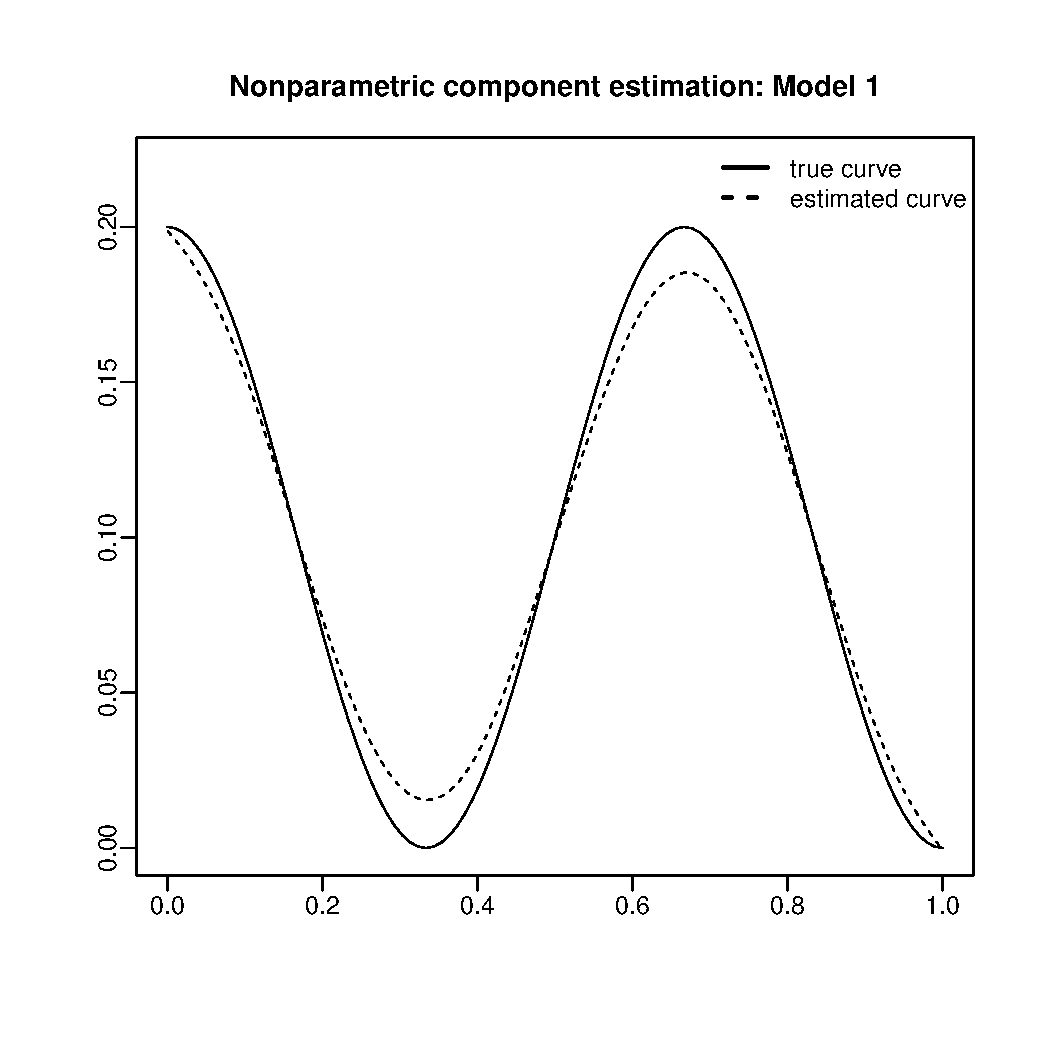
\includegraphics [width=0.4\textwidth]{Fig12_sim1.eps}
		          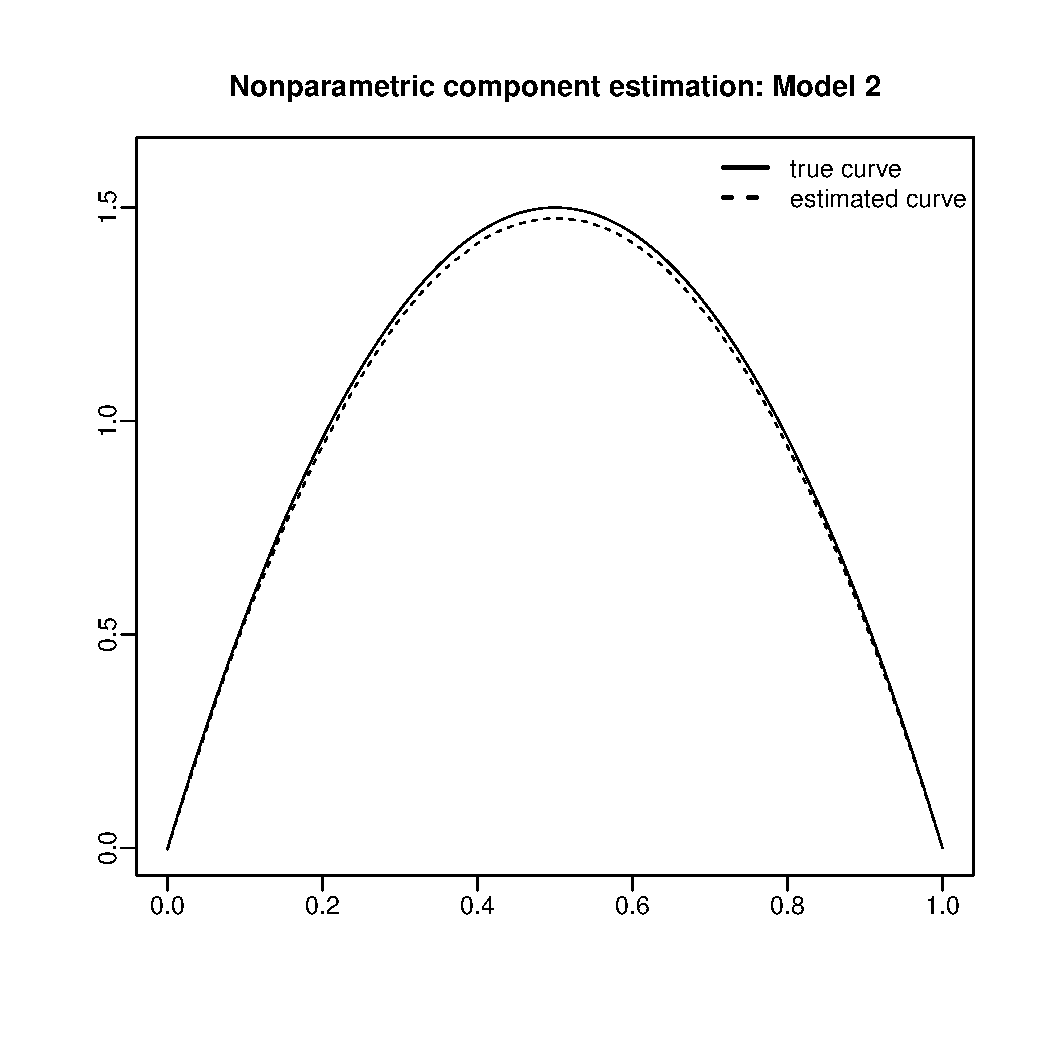
\includegraphics [width=0.4\textwidth]{Fig12_sim2.eps} }
	\caption{Nonparametric component of the regression model,  $m_1(x)$ for Model 1 ({\it left panel}) and $m_2(x)$ Model 2 ({\it right panel}). For all cases, the black line is the true curve and the red line is the averaged estimated curve along the $R=500$ simulated samples.}
	\label{fig:estim_m}
\end{figure}

\section{Model evaluation based on bootstrap methods and the SiZer tool}\label{sec:sizer}

\noindent We are interested in solving hypothesis testing in order to assess the significance of the main effects. Since our main interest is in evaluating the relationship 1/f noise \textit{versus} threshold voltage, $V_{th}$, then we are mainly interested in solving the following testing problem whose null hypothesis is settled as
\begin{equation}\label{eq:H0}
	H_0: \   m'(x)=0, \forall x \in \mathcal{X}; 
\end{equation}
%{\textcolor[rgb]{1,0,0}{\bf {Sugerencia: Podemos usar SiZer!!!}}}
where we denote $x$ any value of $V_{th}$ whose support is $\mathcal{X}$. The null hypothesis of \eqref{eq:H0} asserts that voltage has no effect on noise power level against the alternative that there are regions of non null slope, thus implying a significant effect. 
To solve this testing problem we propose the use of the graphic tool SiZer Map, see for example \cite{GNR2020} to have a detailed description of the SiZer methodology.
%%%%%%%%%%%%%%%%%%%%%%%%%%%%%%%%%%%%%%%%%%%%%%%%%%%%%%%%%%%%%%%%%%%%%%%%%%%%%%%%%%%%%%%%%%%%%%%%%%%%%%%%%%%%%%%%%%%%%%%%%%%%%%%%%%%%%%%
SiZer stands for \textit{significant zero crossings of the derivatives} and was introduced by \cite{CM1999} as a powerful exploratory graphical tool for density and regression functions. This tool uses kernel smoothing to estimate the structure that underlies the data and plays with the smoothing parameter as a scale parameter to visualize the underlying characteristics in the function under study. The characteristics that are not explained by the sample variability, are revealed through the construction of confidence intervals for the first derivative of the function. The main idea of SiZer is to consider the full family of smooths because the estimated curves under different smoothing scales might provide different information on the variation of the curve. 


SiZer methodology relies mainly in a plot that is called the \textit{gradient SiZer map}. First a family of smooth estimators of the target function indexed by the bandwidth parameter is obtained. Second, for gradient SiZer map that displays inference about the first derivative of the curve is developed as follows: for each bandwidth and each value in the support of the curve, a confidence interval for the first derivative is calculated and the sign of the interval is represented on the map using a color code. Considering $n_h$ different bandwidths and $n_x$ estimation points, each pixel in the ($n_x \times n_h$)-map is coded as red if the confidence interval at that estimation point is negative, indicating significant decrease; blue if the confidence interval is positive, indicating
significant increase; purple if zero is within the confidence limits (no significant increase or decrease); and gray indicating regions where the data are too sparse to infer significance.  When a change from blue (red) to red (blue) is detected in the map it means that the underlying curve presents a significant peak (valley) and then the function has a local maximum (minimum).



%%%%%%%%%%%%%%%%%%%%%%%%%%%%%%%%%%%%%%%%%%%%%%%%%%%%%%%%%%%%%%%%%%%%%%%%%%%%%%%%%%%%%%%%%%%%%%%%%%%%%%%%%%%%%%%%%%%%%%%%%%%%%%%%%%%%%%%
\subsection{The SiZer Map Algorithm}
In this section we propose to graphically test whether there is a significant effect of switching voltage on the noise observed in a transistor. The graphical test is based on scale and space inference and is outlined in the following (see \cite{CM1999} and  \cite{GNR2020} for details). For a given $h$ bandwidth and a given value $x$ we construct the estimator detailed in Section \ref{sec:model}, then we obtain an estimation of the derivative $\widehat{m}'(x)$. To develop the SiZer methodology we need to construct confidence intervals around $m'(x)$, and then we need an estimation of the variability of the estimator of the slope. We propose a bootstrap procedure for estimating the variance of $\widehat{m}'(x)$. \

Fix a value $\alpha \in (0,1)$ and let $z_{\alpha/2}$ the quantile of order $1-\alpha/2$ of the Normal(0,1) distribution. For a given bandwidth $h$ and a given value $x$, construct the local-linear estimate of the slope at point $x$, $m'(x)$, that is, obtain the corresponding $\widehat{\beta}_{1,h}(x)=\widehat{m}'_h(x)$,as explained in \ref{sec:backfit}. Then construct the confidence interval (CI) for the slope at point $x$ with a confidence level of $1-\alpha$ following the algorithm below.

\subsubsection*{Algorithm 2}
\begin{enumerate}
	%\item Construct the local-linear estimate of the curve $\widehat{\beta}_{0,h}=\widehat{m}(x)$ and the slope $\widehat{\beta}_{1,h}=\widehat{m}'_h(x)$ as explained in \ref{sec:backfit};
	\item[Step 1.] Run Algorithm 1 to obtain the local-linear estimation $\widehat{m}_h(x_i)$ at each observation point $x_i$, and compute the residuals ${\epsilon}_{ij}=y_{ij}-\widehat{m}(x_i)-\widehat{b}_j-\widehat{\gamma}_i$, for $i =1,\ldots, n$; and, $j=1,2,3$; 
	
	\item[Step 2.] Randomly draw residuals following \cite{MG2015}, and obtain $\epsilon_{ij}^*$ (bootstrap residuals);
	
	\item[Step 3.] Use the re-sampled residuals to generate new response vectors from the predicted values of the fitted model. That is, define: $y_{ij}^*=y_{ij}+\epsilon_{ij}^*$, for $i=1,2,\ldots, n$ and $j=1,2,\ldots, J$;
	
	\item[Step 4.] For each bootstrap sample $\{y_{ij}^*\}$, fit a regression model as in \ref{sec:backfit}, and also obtain the estimation of the slope at point $x$, that is $\widehat{m}'_h(x)^{(1)}$;
	
	\item[Step 5.] Repeat steps 1-4, a total of $R$ times. As a result, obtain a sample $\widehat{m}'_{h}(x)^{(1)}, \widehat{m}'_{h}(x)^{(2)},\ldots, \widehat{m}'_{h}(x)^{(R)}$, for the fixed values $x$, and $h$;
	
	\item[Step 6.] Define the bootstrap standard deviation of the estimator of the slope at $x$ as  $\sigma_{boot,h}(x)$ calculated as the empirical standard deviation of bootstrap sample of slope values, and define the bootstrap CI at level of confidence of $1-\alpha$ as:
	\[
	\left(\widehat{m}'_h(x) -z_{\alpha/2} \sigma_{boot,h}(x), \widehat{m}'_h(x) +z_{\alpha/2} \sigma_{boot,h}(x)\right),
	\]
	for $x$ and $h$ fixed.
\end{enumerate}

Define a grid with a total of $n_x$ locations, that is values of $x$, and a grid of bandwidths $h$ of size $n_h$ and construct the SiZer Map following the color code explained above.

Figures \ref{fig:sizer1}-\ref{fig:sizer4} shows the results obtained for the data on 1/f noise. Figure \ref{fig:sizer1} displays a clear region of red pixels which means a decreasing trend of the noise power level with the value of voltage at least for the intermediate values. In this case, we cannot keep the assertion in $H_0$ given in \eqref{eq:H0} which is rejected, in consequence, we conclude that, at this bias condition, there is a positive correlation between threshold voltage and noise power level.

Figure \ref{fig:sizer2} shows a map completely purple, which means that no regions in the support of $V_{th}$ have been found where the slope can be rejected to be 0, that is, no features are detected at any location ($x$) or scale ($h$). The null hypothesis in \eqref{eq:H0} cannot be rejected with the data at hand. The conclusion is that at these bias conditions, i.e. $V_d=1$v, $V_g=0.5$v, the threshold voltage does not have any influence in the noise registered. These two cases are in well concordance with the plots seen in Figures \ref{fig:backfit1} and \ref{fig:backfit2}.

However, the results displayed in Figures  \ref{fig:sizer3} and \ref{fig:sizer4} seems to contradict the ones observed in Figures \ref{fig:backfit3} and \ref{fig:backfit4}. The two SiZer maps suggest that the relationship voltage-noise is first increasing and later decreasing, since we appreciate a clear change from blue to red in both figures. This change of trend is also appreciated in Figures \ref{fig:backfit3} and \ref{fig:backfit4}, but there we can also see that the curve in both cases tends to increase on the right edge of the plot, suggesting that the noise power level is increasing for the highest threshold voltages. After a deeper examination of the plots in Figures \ref{fig:backfit3} and \ref{fig:backfit4},  we see that this increasing tendency in both curves is only supported by two data points in each case, we can justify the increase by a mere boundary effect and not by a true characteristic of the curve. This reasoning is confirmed looking at the corresponding SiZer maps in  Figures  \ref{fig:sizer3} and \ref{fig:sizer4} where we see that a gray region is plotted on the right edge of the map, revealing that the sparse of data on that region does not allow us to get any clear conclusion about the behavior of the curve there. So, in these two cases, the only change of tendency of the relationship voltage-noise is the change from  increasing to decreasing which is clearly reflected in the corresponding SiZer maps as well as in Figures \ref{fig:backfit3} and \ref{fig:backfit4}, where a unique estimation of the curve (that is only one $h$ value) is considered.

\begin{figure}[ht]
	\centerline{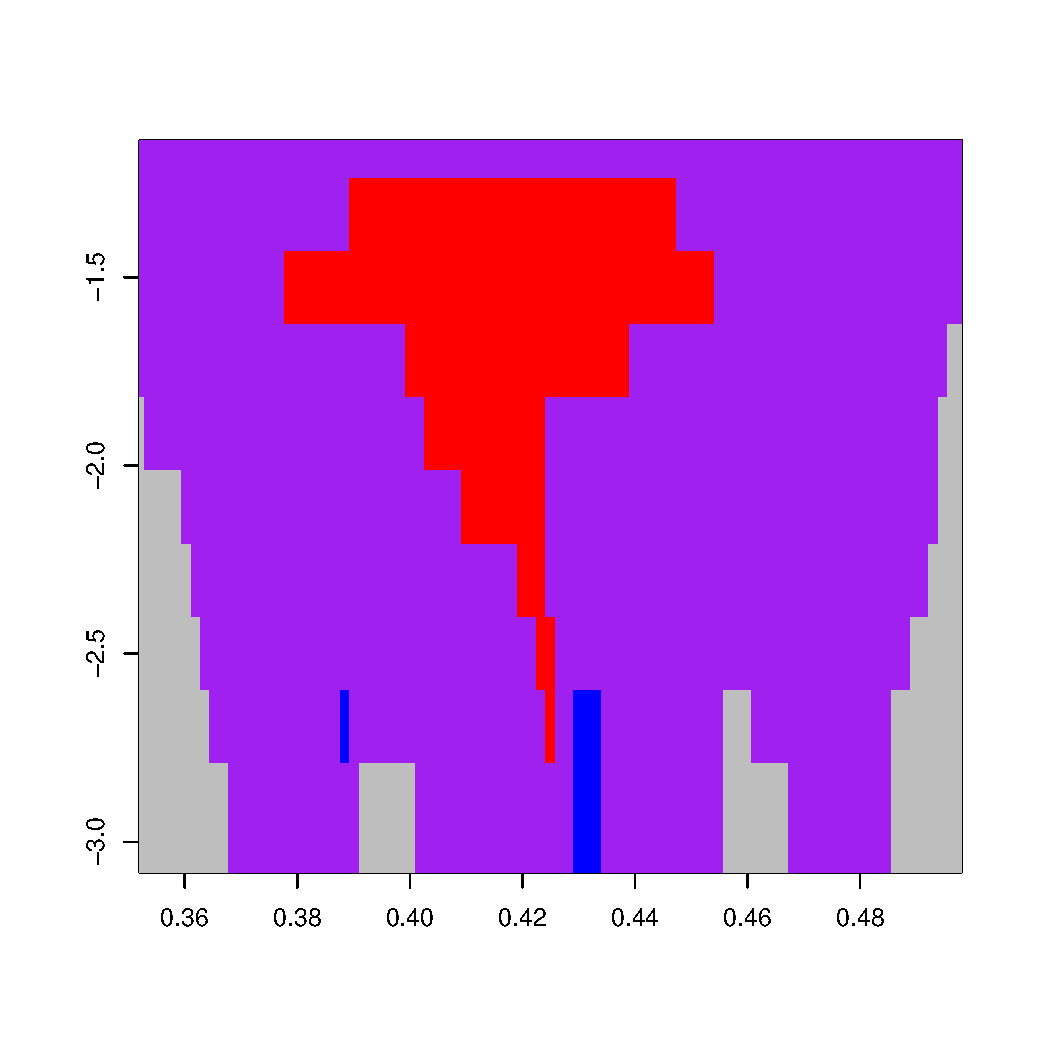
\includegraphics [width=0.6\textwidth]{Fig13_sizerd05g05.eps}}%{backfit_g1.eps} }
	\caption{SiZer map based on the sample of $DIE$s at bias conditions $V_d=V_g=0.5$v. }
	\label{fig:sizer1}
\end{figure}
\begin{figure}[ht]
	\centerline{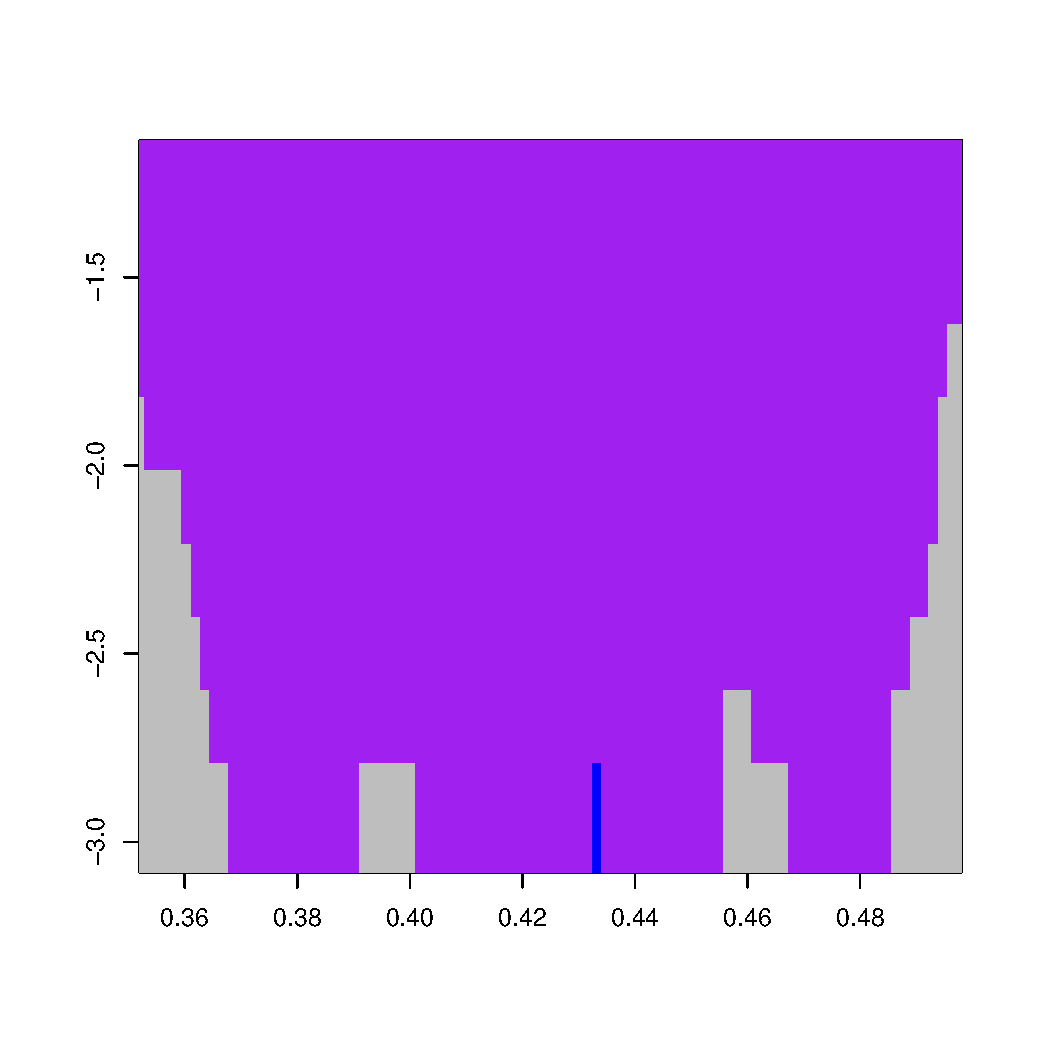
\includegraphics [width=0.6\textwidth]{Fig14_sizerd1g05.eps}}%backfit_g2.eps} }
	\caption{SiZer map based on the sample of $DIE$s at bias conditions $V_d=1$v, $V_g=0.5$v.}
	\label{fig:sizer2}
\end{figure}
\begin{figure}[ht]
	\centerline{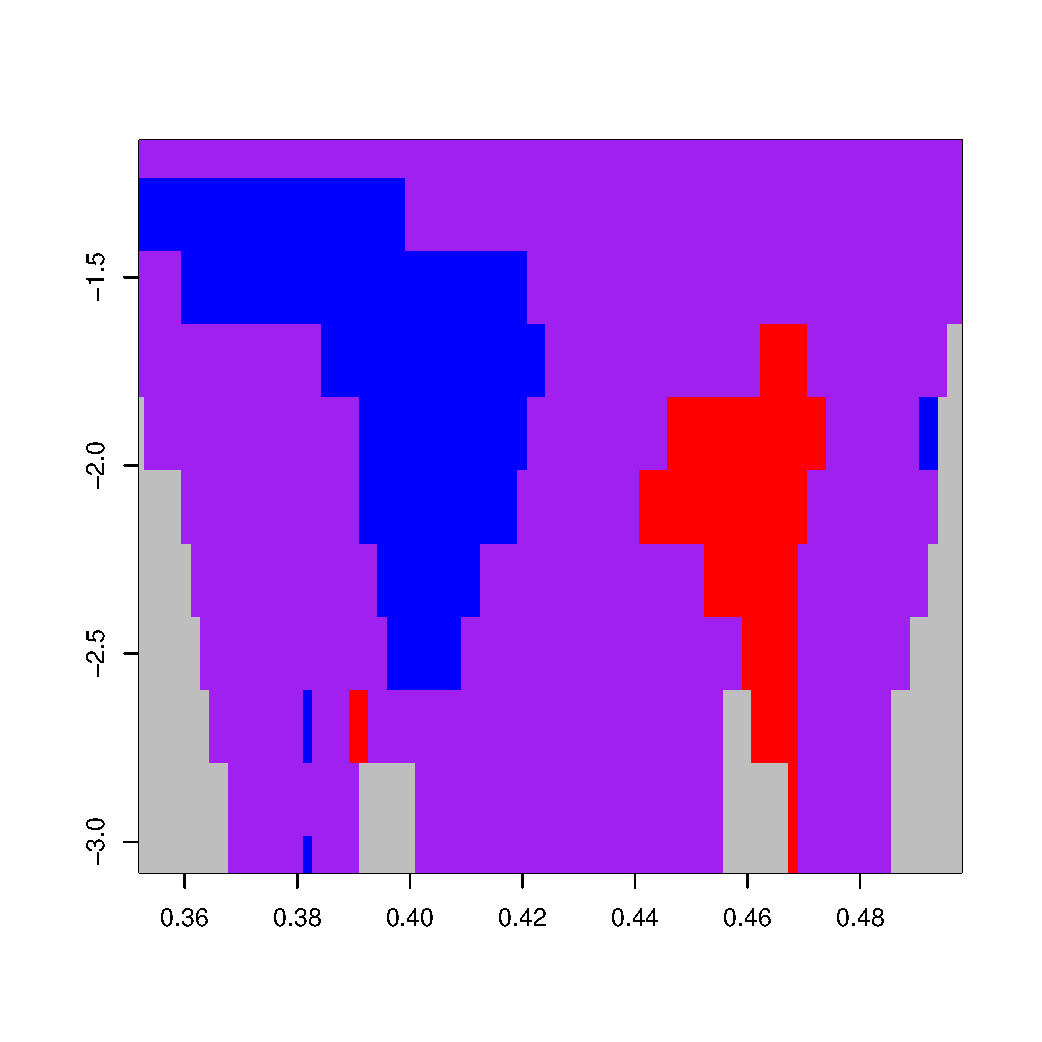
\includegraphics [width=0.6\textwidth]{Fig15_sizerd05g1.eps}}%{backfit_g3.eps} }
	\caption{SiZer map based on the sample of $DIE$s at bias conditions $V_d=0.5$v, $V_g=1$v.}
	\label{fig:sizer3}
\end{figure}
\begin{figure}[ht]
	\centerline{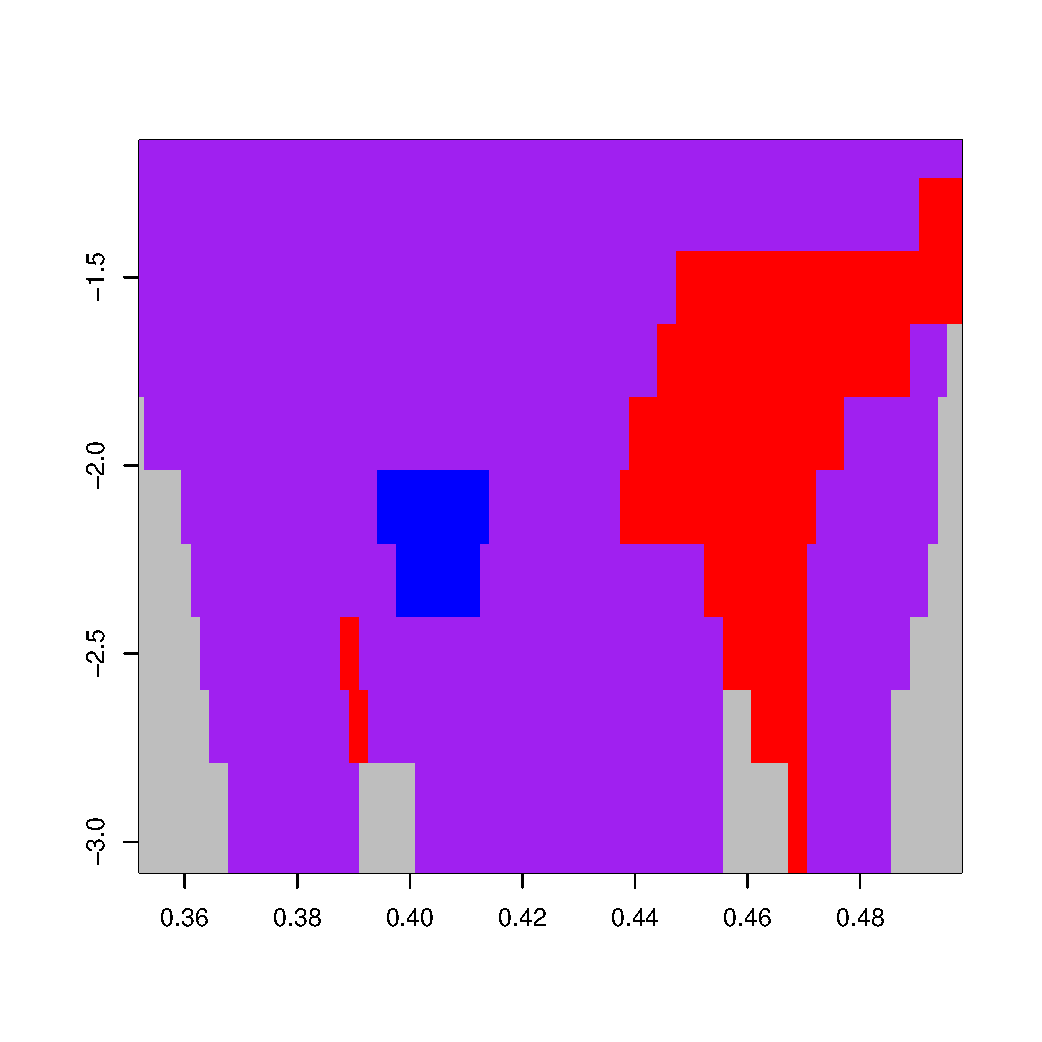
\includegraphics [width=0.6\textwidth]{Fig16_sizerd1g1.eps}}%{backfit_g4.eps} }
	\caption{SiZer map based on the sample of $DIE$s at bias conditions $V_d=V_g=1$v.}
	\label{fig:sizer4}
\end{figure}
%%%%%%%%%%%%%%%%%%%%%%%%%%%%%%%%%%%%%%%%%%%%%%%%%%%%%%%%%%%%%%%%%%%%%%%%%%%%%%%%%%%%%%%%%%%%%%%%%%%%

\section{Conclusion}\label{sec:concl}

Our motivation for this paper is the analysis of potential correlations between spectral noise current and threshold voltage measured on common on-wafer MOSFETs. A deep exploratory analysis of the data reveals that it is inappropriate to assume the assumptions that hold the classical Normal linear model nor the ANOVA version that allows accounting for dependency structures resulting from a repeated measures design. More sophisticated methods have been required to properly analyze the data and reach reliable conclusions.
We have designed and run an algorithm based on modern nonparametric statistics and graphical tools that help in the interpretation and understanding of the nature of the data. In particular we have built a mixed-effect model with a nonparametric component to explain the main relationship of the model that is the effect of threshold voltage $V_{th}$ on spectral noise current, $Noise$ which is considered in the frequency domain. Our method is an adaptation of the backfitting algorithm to our particular requirements. Afterwords, we have proposed 
graphical test developed through scale and space inference about the slope of the nonparametric component of the model. Punctual  confidence intervals have been constructed around the curve and for different levels of smoothing (bandwidths). The graphical representation allows one to detect and confirm regions where the relation between the two magnitudes, $V_{th}$ and $Noise$, is increasing, decreasing or nonexistent. For the four datasets considered the results obtained reflect different behaviors of the variable $Noise$ with respect to the variable $V_{th}$ depending on the particular combination of the bias condition considered.
Although there are important contributions in the recent literature for explaining the random behavior of low frequency noise, to our knowledge, there are not many studies specifically focused on the relationship noise-voltage from a statistical learning point of view, that is, based on data. This is where the statistician can be of great help in order to customize powerful machine learning techniques making them useful to solve problems in particular in this area of Electronic Engineering.  


\bmhead{Acknowledgments}
The authors thank the Laboratory of Nanoelectronics in the Research Centre for Information and Communications Technologies (CITIC-UGR) at the University of Granada (Spain) for providing the data for the study. This work was supported in part by the Spanish Ministry of Science and Innovation through grants number	RTI2018-099723-B-I00, and PID2020-120217RB-I00.


\section*{Declarations}
%
%Some journals require declarations to be submitted in a standardised format. Please check the Instructions for Authors of the journal to which you are submitting to see if you need to complete this section. If yes, your manuscript must contain the following sections under the heading `Declarations':

\begin{itemize}
%\item Funding: 
%\item Conflict of interest/Competing interests (check journal-specific guidelines for which heading to use): No
\item Availability of data and material: Available from authors.
\item Code availability: Available from authors.
\item Authors' contributions: All authors contributed equally to this work
\item Ethics approval: Not applicable.
\item Consent to participate: All authors have expressed their consent to participate.
\item Consent for publication: All authors have expressed their consent for publication.
%
\end{itemize}





\bibliography{sn-bibliography}% common bib file
%% if required, the content of .bbl file can be included here once bbl is generated
%%\input sn-article.bbl

%% Default %%
%%\input sn-sample-bib.tex%


\begin{thebibliography}{00}
	
	\bibitem{Betal2016} Banaszeski da Silva, M., Tuinhout, H.P., Zegers-van Duijnhoven, A..  Wirth, G.I. and Scholten, A.J. (2016). A Physics-Based Statistical RTN Model for the Low Frequency Noise in MOSFETs,  {\it IEEE Transactions on Electron Devices}, {\bf 63}, (9), 3683--3692.
	
	
	
	\bibitem{BHN2000} Berkovits, I., Hancock, G.R., and Nevitt, J., (2000), Bootstrap Resampling Approaches for Repeated Measure Designs: Relative Robustness to Sphericity and Normality Violations, Educational and Psychological Measurement,  60 (6), 877--892 
	
	
	\bibitem{Betal2020} Both, T.H., Banaszeski da Silva, M., Wirth, G.I., Tuinhout, H.P., Zegers-van Duijnhoven, A., Croon, J.A. and Scholten, A. J., (2020). An Overview on Statistical Modeling of Random Telegraph Noise in the Frequency Domain.  In: Grasser T. (eds) {\it Noise in Nanoscale Semiconductor Devices}. Springer, Cham. $https://doi.org/10.1007/978-3-030-37500-3_15$
	
	\bibitem{BHT1989} Buja, A., Hastie, T. and Tibshirani, R. (1989). Linear Smoothers and Additive Models. {\it The Annals of Statistics} {\bf 17} (2), 453--510.
	
	\bibitem{CM1999} Chaudhuri, P. and Marron, J.S. (1999), SiZer for Exploration of Structures in Curves. {\it Journal of the American Statistical Association}, {\bf 94}(447), 807–-823.
	
	\bibitem{DG2003} Davidian, M. and Giltinan, D.M. (2003), Nonlinear models for repated measurement data: An overview and update. {\it Journal of Agricultural, Biological and Environmental Statistics}, {\bf 8}, 387--419. 
	
	\bibitem{Duty2016} Duty, R.. (2016). On-wafer investigation of spectral noise and threshold voltage correlation on 28 nm and beyond MOSFETs, Masterthesis, University of Applied Sciences Munster
	
	\bibitem{FG1996}  Fan, J. and Gijbels, I. (1996). {\it Local Polynomial Modelling and Its Applications}. Chapman \& Hall/CRC
	
	
	\bibitem{GNR2020} Gamiz, M.L., Nozal-Ca\~nadas, R. and Raya-Miranda, R. (2020). TTT-SiZer: A graphic tool for aging trends recognition, {\it Reliability Engineering and System Safety}, {\bf 202}, 1--17.
	
	\bibitem{HT1990} Hastie, T., and Tibshirani, R. (1990), {\it Generalized Additive models}. CHAPMAN \& HALL/CRC.
	
	\bibitem{HKHC1990} Hung, K. K., Ko, P.K., Hu, C. and Cheng, Y.C., (1990). A unified model for the flicker noise in Metal-Oxide-Semiconductor Field-Effect Transistors, {\it IEEE Transactions on Electronic Devices}, {\bf 37} (3), 654--665.
	
	\bibitem{MG2015} Modugno, L. and Giannerini, S., (2015). The wild bootstrap for multilevel models, {\it Communications in Statistics—Theory and Methods}, {\bf 44} (22), 4812-–4825.
	
	\bibitem{OR1997} Opsomer, J.D., Ruppert, D. (1997). Fitting a bivariate additive model by local polynomial regression. {\it Annals of Statistics}, {\bf 25} (1), 186 -- 211.
	
	\bibitem{Opsomer2000} Opsomer, J.D. (2000). Asymptotic Properties of Backfitting Estimators. {\it Journal of Multivariate Analysis}, {\bf 73} (2),  166--179.
	
	\bibitem{PB2000} Pinheiro, J.C. and Bates, D.M. (2000) {\it Mixed-Effects Models in S and S-PLUS}, Springer.
	
	\bibitem{Petal2019} Puschkarsky, K., Grasser, T., Aichinger, T., Gustin, W., Reisinger, H. (2019), Review on SiC MOSFETs High-Voltage Device Reliability Focusing on Threshold Voltage Instability, {\it IEEE Transactions on Electron Devices}, {\bf 66} (11), 4604--4616.
	
	\bibitem{R2021}
	R Core Team (2021). R: A language and environment for statistical computing. R Foundation for Statistical Computing, Vienna, Austria. URL
	https://www.R-project.org/.
	
	
	\bibitem{RMGRO2016} Rodriguez, N., Marquez, C., Gamiz, F., Ruiz, R. and Ohata, A.,(2016).  Electrical characterization of Random Telegraph Noise in Fully-Depleted Silicon-On-Insulator MOSFETs under extended temperature range and back-bias operation, {\it Solid-State Electronics}, {\bf 117}, 60--65.
	
	\bibitem{Schroder2006} Schroder, D.K. (2006). Semiconductor materials and devices characterization. John Wiley and Sons, Inc.
	
	
	\bibitem{Tetal2015} Theodorou, C.G., Ioannidis, E.G., Haendler, S., Planes, N., Josse, E., and Dimitriadis, C.G. (2015). New LFN and RTN analysis methodology in 28 and 14nm FD-SOI MOSFETs. {\it Conference: IEEE International Reliability Physics Symposium (IRPS)}
	
	
	\bibitem{Tsividis1998} Tsividis, Y. (1998). Operation and Modelling of the MOS Transistor, Oxford University Press.
	
	\bibitem{WL2004} Wu, H. and Liang, H. (2004). Backfitting random varying-coefficient models with time-dependent smoothing covariates, {\it Scandinavian Journal of Statistics}, {\bf 31} (1), 3--19.
	
	\bibitem{WK2020} Wu, T.L. and Kutub, S.B. (2020). Machine Learning-Based Statistical Approach to Analyze Process Dependencies on Threshold Voltage in Recessed Gate AlGaN/GaN MIS-HEMTs, {\it IEEE Transactions on Electron Devices}, {\bf 67} (12), 5448--5453.
	% etc
	
	
\end{thebibliography}


\end{document}
